\documentclass[a4paper,10pt]{article}
\usepackage[left=2.2cm,right=2.2cm,top=2.5cm,bottom=2.5cm]{geometry}
\usepackage{parskip}
\usepackage{graphicx}
\usepackage{float}
\usepackage[hidelinks]{hyperref}
\usepackage{cleveref}
\usepackage{xurl}

\graphicspath{{../images}}

\begin{document}

% Title
\begingroup
\centering
\LARGE Multivariable Calculus Self-Learning Module\\[1em]
\large Setup \& Usage Manual\\[4\baselineskip]
\endgroup

\tableofcontents

\clearpage

\listoffigures

\clearpage

\section{Introduction}

The website is currently hosted for free by \emph{GitHub Pages}. In order to deploy a website using GitHub Pages you need a \emph{GitHub} account. 

\paragraph{What is GitHub?} GitHub is a popular, free, cloud-based platform that allows users to store and share files. It is mainly (but not exclusively) used for collaboration on coding projects. Think of it as a storage space just like Google Drive for anything you might want to share with others. Each project on GitHub is stored in its own directory, which is called a \emph{repository}. GitHub uses \emph{Git} to keep track of any changes that happen in a repository.

\paragraph{What is Git?} Git is an open-source version control software which is widely used to keep track of any changes that happen in a file. Think of it as an alternative to making multiple files such as: ``exam-v1'', ``exam-v2'', ``exam-v2-fixed'', \dots, ``exam-final''. Git keeps track of all the different versions for you, and it lets you revert back to any previous version of your file, or test stuff by creating a new version branch without ever affecting your main branch. GitHub uses Git, but Git is independent of GitHub and it works with its own local repositories on your computer.

\paragraph{How does GitHub Pages work?} You simply deploy your website directly from your GitHub repository on GitHub Pages. After that point, your website is always running, and whenever you make a change to the repository, it will be implemented almost immediately on the live website.

\paragraph{What is the point of all this?} The idea is the following:
\begin{enumerate}
    \item You keep your own version of the website on your computer, along with a local installation of Git.
    \item Say you make some changes that you are happy with, e.g.\ you add an exercise or fix a mistake. You \emph{commit} the changes to your local Git repository.
    \item You then \emph{push} the local Git repository to the online GitHub repository.
    \item GitHub Pages will automatically detect the new changes from your GitHub repository and deploy a new version of your website.
\end{enumerate}
The good part is that once set up this process is totally free, standardised, relatively easy, and should be familiar to anyone who has ever collaborated on a coding project. 

\paragraph{Python script.} A Python script that can split and convert a \LaTeX\ document into HTML exercise files is also provided.

\clearpage
\section{Setup}

Setup is a bit long but at least you only have to do it once.

\subsection{Git}

The latest version of Git for Windows can be downloaded from:

\url{https://git-scm.com/download/win}

In the vast majority of cases the 64-bit version (first link) is required. The default installation options are fine. After installation is done, check if Git has been installed correctly by opening a terminal (can be done by \emph{Windows key + X} $>$ \emph{Terminal (Admin)}) and typing the command: 

\texttt{git -v}

The response should be the latest version of Git (e.g.\ \Cref{fig:git-v}). 

\begin{figure}[htbp]
    \centering
    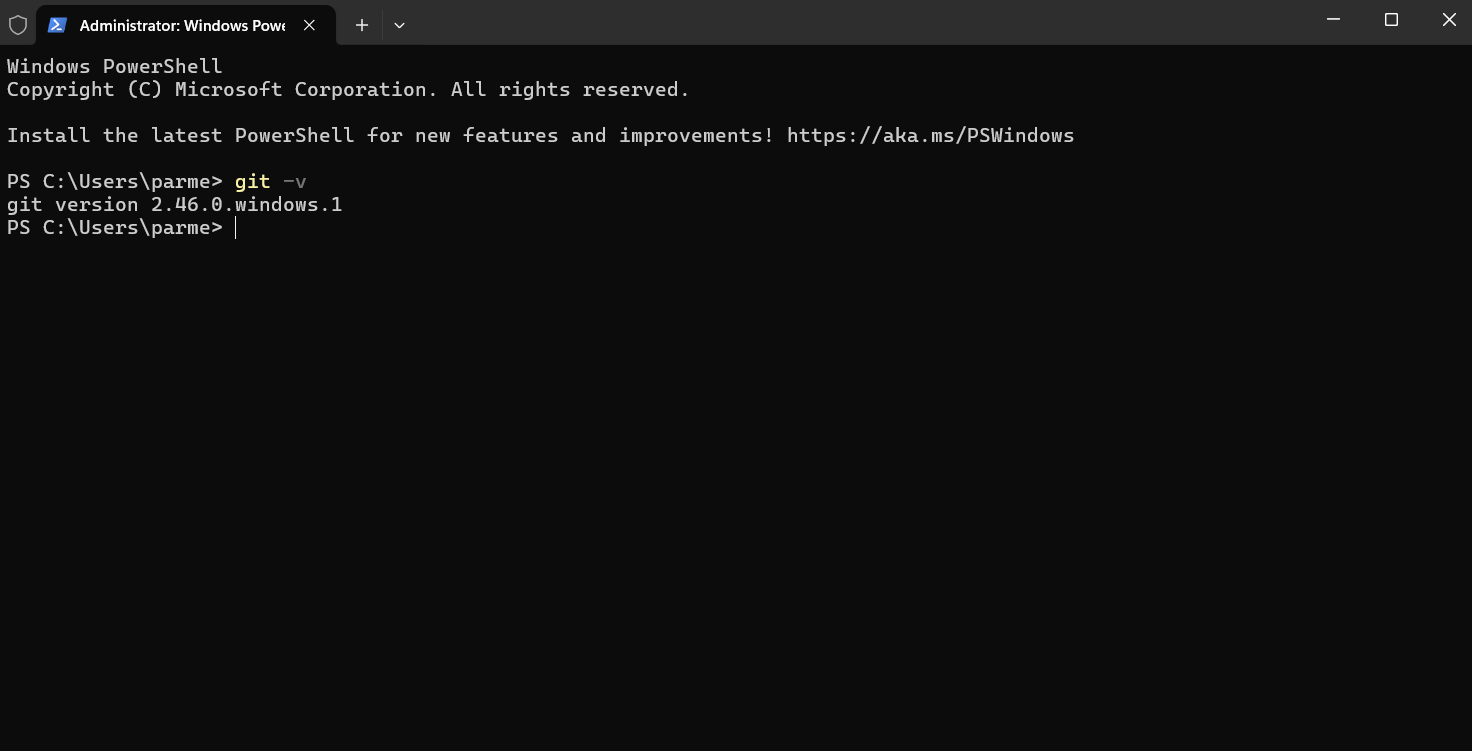
\includegraphics[width=\textwidth]{git-v.png}
    \caption{\texttt{git -v}}
    \label{fig:git-v}   
\end{figure}

If not, try restarting the computer and check again. Restart is sometimes needed so that folder in which Git is installed is permanently added to the Windows PATH variable, which lets Windows know what the \texttt{git} command means. If this also doesn't work, Git must be added to the PATH manually. This is annoying and should (and most likely will) not happen, and at that point it is probably best to Google something like ``add git to path windows 11'' (or whatever your Windows version is) and follow the detailed instructions.

\subsubsection{Initiating a local Git repository}
\label{sec:git_init}

Assuming that Git is already installed, there are two ways to initiate a local Git repository.

\paragraph{Option 1: Initiate a new Git repository for an existing local directory.} Suppose you have the directory \emph{mvc-self-learning-module} somewhere on your computer and it is not already associated with a local Git repository. In order to initiate one, you can open the directory in a terminal (can be done by navigating within the directory using the File Explorer, and then on any empty space \emph{Right click} $>$ \emph{Open in Terminal}) and then type the command: 

\texttt{git init}

The output should be something like \Cref{fig:git_init}.

\begin{figure}[htbp]
    \centering
    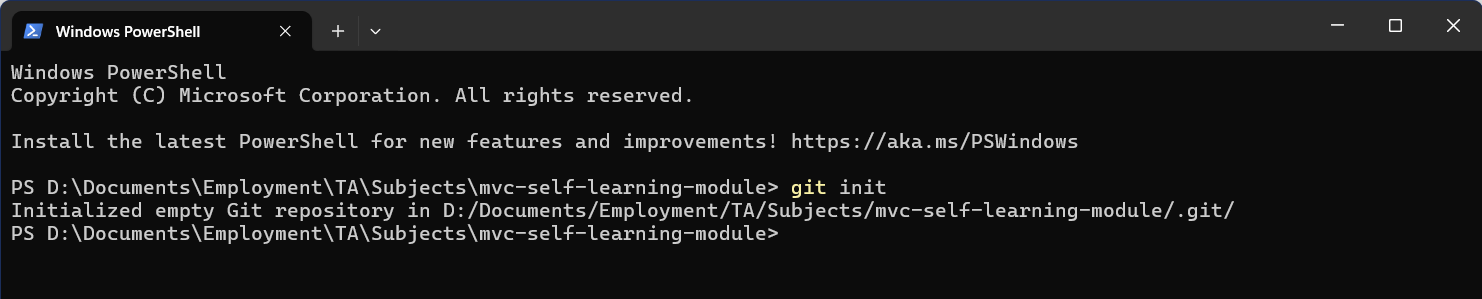
\includegraphics[width=\textwidth]{git_init.png}
    \caption{\texttt{git init}}
    \label{fig:git_init}   
\end{figure}


You can visually inspect the Git repository if you enable the option of seeing the hidden files on your computer (can be switched on within the File Explorer itself from \emph{View} $>$ \emph{Show} $>$ \emph{Hidden items} (\Cref{fig:hidden_items})). In that case, a folder named \emph{.git} should appear in the current directory, which shows that the directory is now a Git repository (first folder in \Cref{fig:hidden_items}). 

You can now interact with this Git repository anytime by opening the directory (\emph{mvc-self-learning-module}, not \emph{.git}) in a terminal as before.

\begin{figure}[htbp]
    \centering
    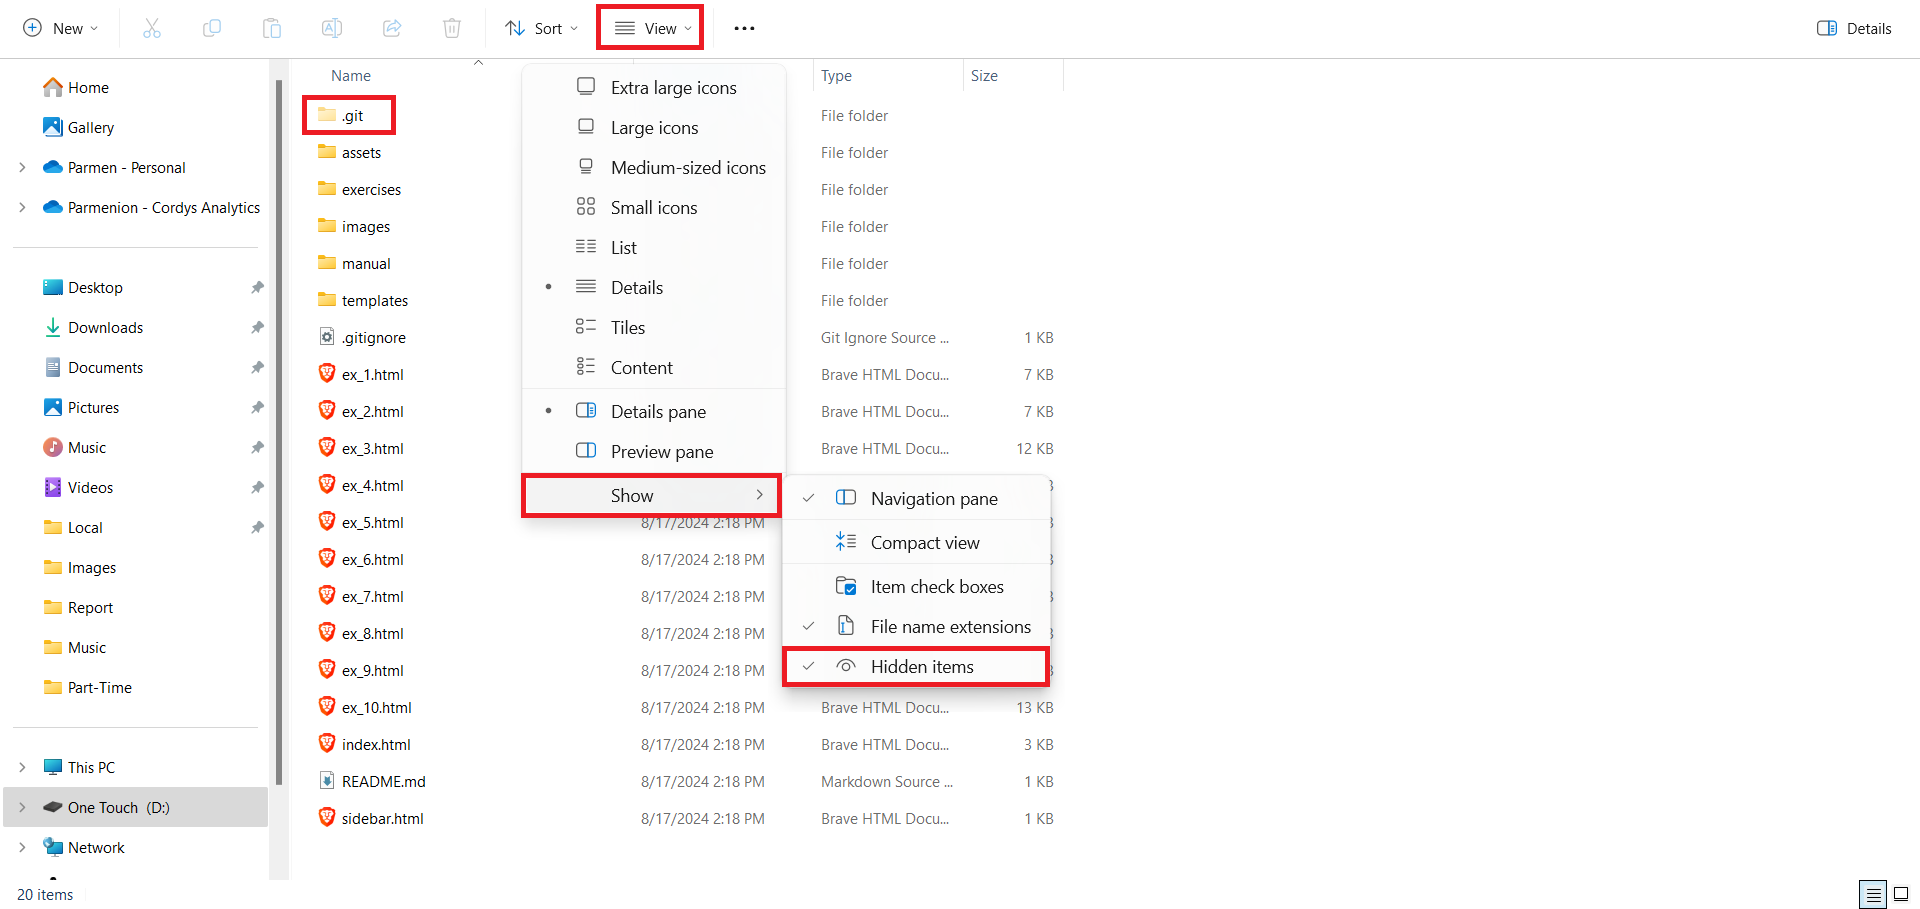
\includegraphics[width=\textwidth]{hidden_items.png}
    \caption{Enable hidden items. .git folder is shown.}
    \label{fig:hidden_items}   
\end{figure}

\paragraph{Option 2: Clone an already existing Git repository from GitHub.} This can be done as follows:
\begin{enumerate}
    \item Copy the link to the repository from your browser, e.g.: 

    \url{https://github.com/StefanMaubach/mvc-self-learning-module}
    
    \item Navigate to the location on your computer where you would like to store the local Git repository and open a terminal within this location (\emph{Right click} $>$ \emph{Open in Terminal}).
    
    \item Type the command:

    \texttt{git clone https://github.com/StefanMaubach/mvc-self-learning-module}
\end{enumerate}
The repository should then appear in a new directory named \emph{mvc-self-learning-module} in the desired location. 

In order to further interact with the Git repository you need to access this new directory with the terminal. You can enter the directory through the File Explorer and then open a new terminal in this directory in the same way as before, or if you still have the previous terminal open, you can access the new directory with the following command:

\texttt{cd mvc-self-learning-module}

(cd is the command used by Windows as well as Unix based systems to \textbf{c}hange \textbf{d}irectory). To verify that you cloned the repository correctly, you can check its status with the following command:

\texttt{git status}

Throughout the above process, the terminal output should look something like \Cref{fig:git_clone}.

\begin{figure}[htbp]
    \centering
    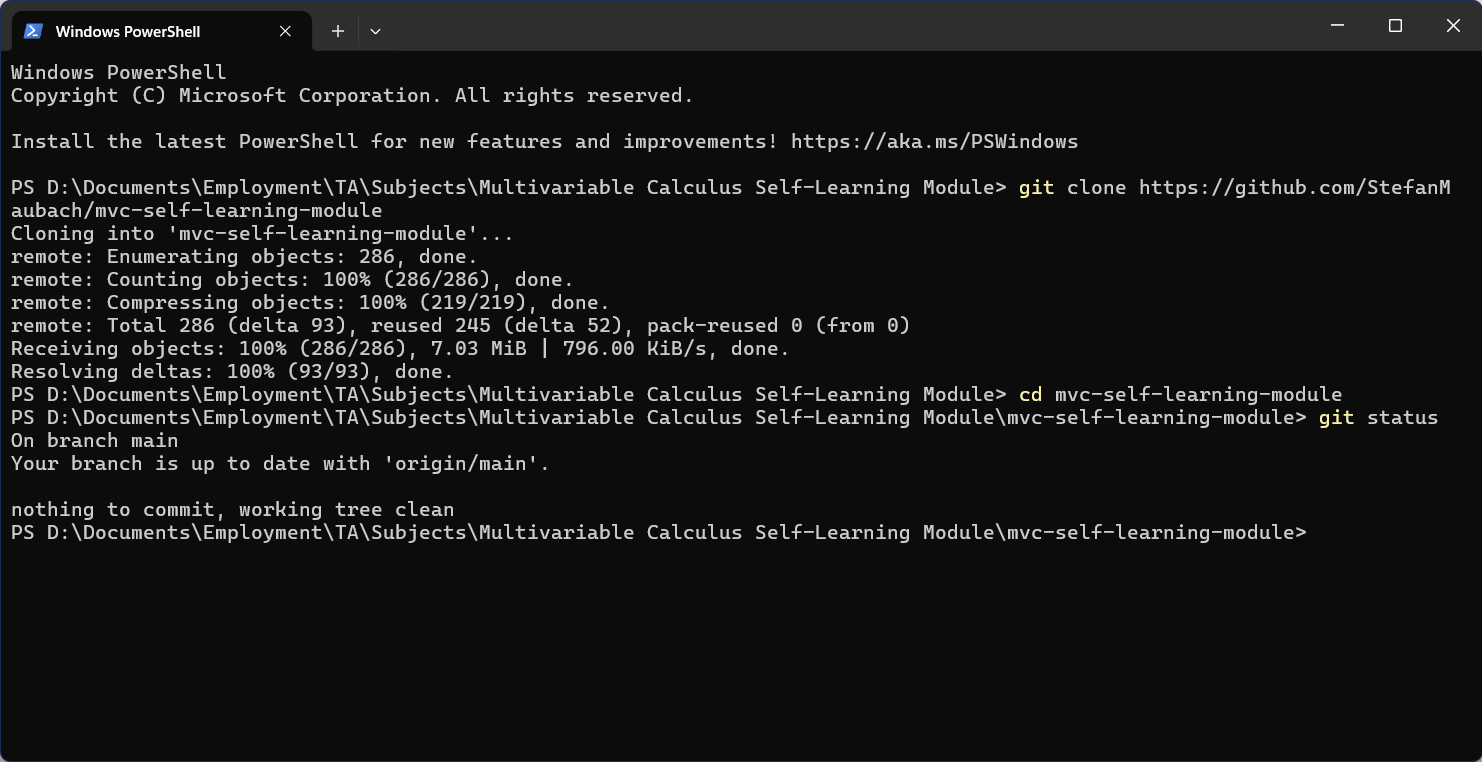
\includegraphics[width=\textwidth]{git_clone.png}
    \caption{Clone a GitHub repository.}
    \label{fig:git_clone}   
\end{figure}


\subsubsection{Making the first commit}
\label{sec:first_commit}

I now assume that you have a local Git repository. You now probably want Git to make a checkpoint out of the current state of your files by making a \emph{commit}. This involves the following two steps:
\begin{itemize}
    \item You tell Git what you want it to keep track of by using the command \texttt{git add}, followed by whatever filenames you want to add. In the vast majority of cases you probably want to add all of the files (except those from \emph{.gitignore}, see \Cref{sec:gitignore}) by using the dot (.) character. So the full command is:

    \texttt{git add .}

    You can ignore any warnings of the form ``$X$ will be replaced by $Y$ the next time Git touches it'' if they appear.

    \item Now it is time to finalise the commit by using the command \texttt{git commit}. Git by default asks you to label your commit by a message which briefly describes what the commit is about, e.g.\ ``ex\_1001 added'' or ``new sidebar layout'' etc. For the first commit though it is not uncommon to choose a less descriptive message, such as ``first commit'' or something. The messages are added using the \texttt{-m} flag. So the full command would look something like:

    \texttt{git commit -m "first commit"}    
\end{itemize}
The terminal output should look similar to \Cref{fig:first_commit}.

\begin{figure}[htbp]
    \centering
    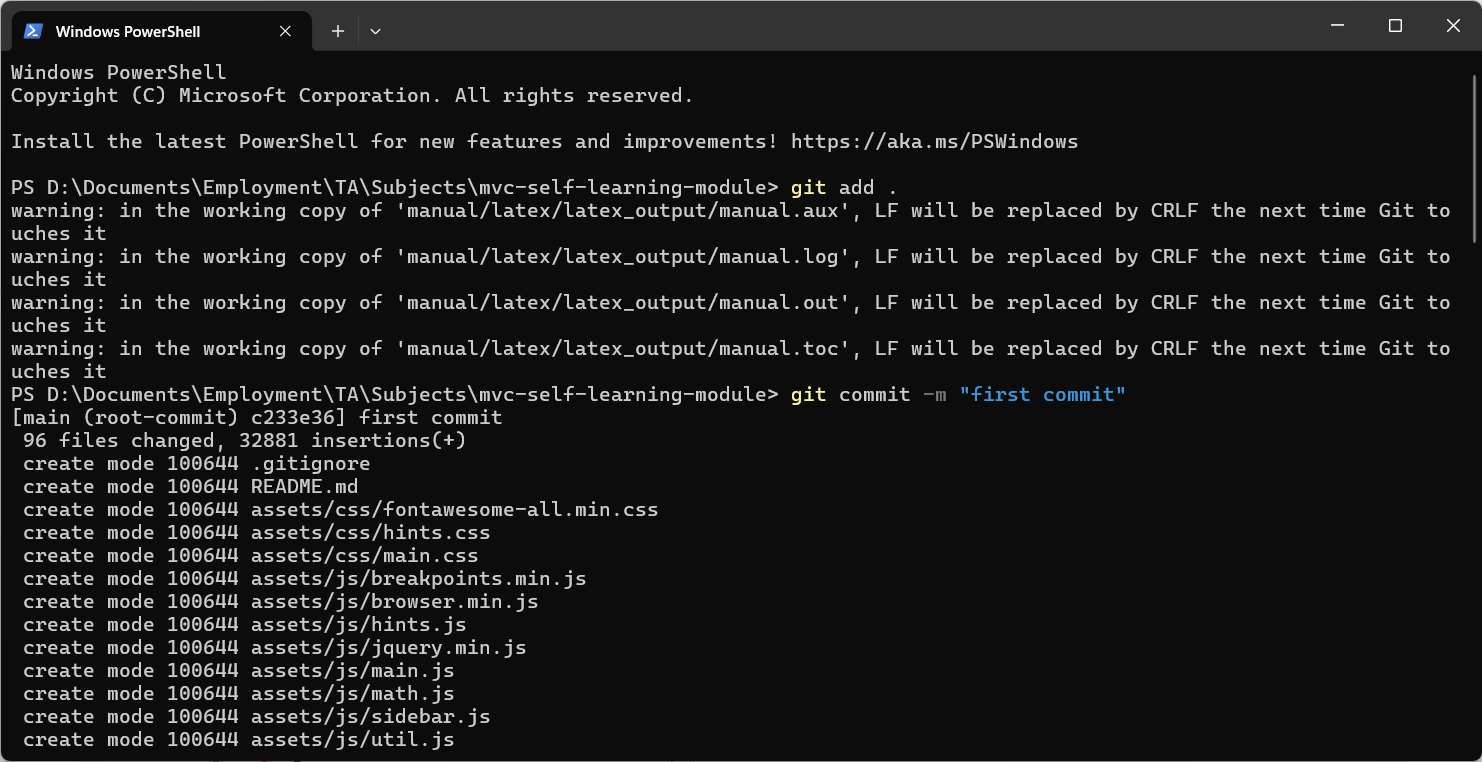
\includegraphics[width=\textwidth]{first_commit.png}
    \caption{First commit.}
    \label{fig:first_commit}   
\end{figure}

\paragraph{Identity verification.} If you have cloned a GitHub repository (Option 2 from \Cref{sec:git_init}), Git may throw an error and ask you to verify your identity before accepting the commit. The error will ask you to run the following commands:

\texttt{git config --global user.email "you@example.com"}

\texttt{git config --global user.name "Your Name"}

Run these commands, replacing \texttt{you@example.com} by the email you used to sign up with GitHub, and \texttt{Your Name} by your GitHub username (include the \texttt{"\dots"}). Most likely you will only have to do this once. When this is done, try committing your changes again.

\subsubsection{Adding .gitignore and README.md files (optional)}
\label{sec:gitignore}

If a Git repository is to be shared with others, it is a good idea for it to contain a \emph{.gitignore} file and a \emph{README.md} file (maybe also a \emph{LICENSE} file if you want to clarify that it is open-source, but that is probably a future concern). It is easiest to create and edit these files locally using VSCode (see \Cref{sec:vscode} for setup). Alternatively, you can create these files as follows:
\begin{enumerate}
    \item Enable file name extensions being shown in the File Explorer by \emph{View} $>$ \emph{Show} $>$ \emph{File name extensions} (right above \emph{Hidden items} in \Cref{fig:hidden_items}).
    \item Create a blank text file in the directory by \emph{Right click} $>$ \emph{New} $>$ \emph{Text Document}. A new text document with a name along the lines of \emph{New Text Document.txt} should appear in the directory.
    \item Now you can simply replace the document's entire filename INCLUDING THE EXTENSION \emph{.txt} by \emph{.gitignore} or \emph{README.md}.
\end{enumerate}
You can edit these files in VSCode, or in Notepad by \emph{Right click} (on the file) $>$ \emph{Open with}, and then either choosing Notepad if it appears as a suggestion, or searching for Notepad through \emph{Choose another app}.

\paragraph{The .gitignore file.} The .gitignore file tells Git what to not keep track of, and therefore also not to share with others. Whatever you add on .gitignore will stay in your local computer, forever invisible to Git. To add a file or even a folder to .gitignore, you simply open the file and write its name in a new row. For example, I have already included a .gitignore in the repository, which currently ignores the local \LaTeX\ artefacts produced in my computer. Perhaps you would also like to add the entire \emph{exercises} folder in the future so that nobody but you has access to the exercises scan/latex/pdf (although someone who is motivated enough can still view the entire exercise through the HTML files themselves).

\paragraph{The README.md file.} The README file is what everyone expects to see as a first introduction to your repository when you share it with them. GitHub by default displays the contents of the README.md file (if it exists) to anyone who accesses your repository through their browser. I have already included a README file in the repository, which only includes a title currently. The \emph{.md} extension means that the file is written in \emph{Markdown}, which is an easy markup language that essentially makes fancy text files. Pretty much all the Markdown formatting you will ever need to write a typical README file can be found here:

\url{https://www.markdownguide.org/cheat-sheet/}


\subsection{GitHub}

Opening a GitHub account should be as straightforward as opening any account in any other service if you select \emph{Sign Up} from: 

\url{https://github.com/}


\subsubsection{Associating the local Git repository with a GitHub repository}

I assume that Git is already installed and that you have a GitHub account. This step needs to be done ONLY IF YOU INITIATED A NEW LOCAL GIT REPOSITORY FOR YOUR LOCAL DIRECTORY (Option 1 in \Cref{sec:git_init}). If you cloned an already existing Git repository from GitHub, you can skip this section.

\paragraph{Creating a new GitHub repository.} If you want to create a new GitHub repository for your project, you can do that by accessing your GitHub profile through your browser, at:

\url{https://github.com/StefanMaubach}

and then navigating to the \emph{Repositories} tab and selecting \emph{New} on the right (e.g.\ on my profile it looks like \Cref{fig:new_repository}).

\begin{figure}[htbp]
    \centering
    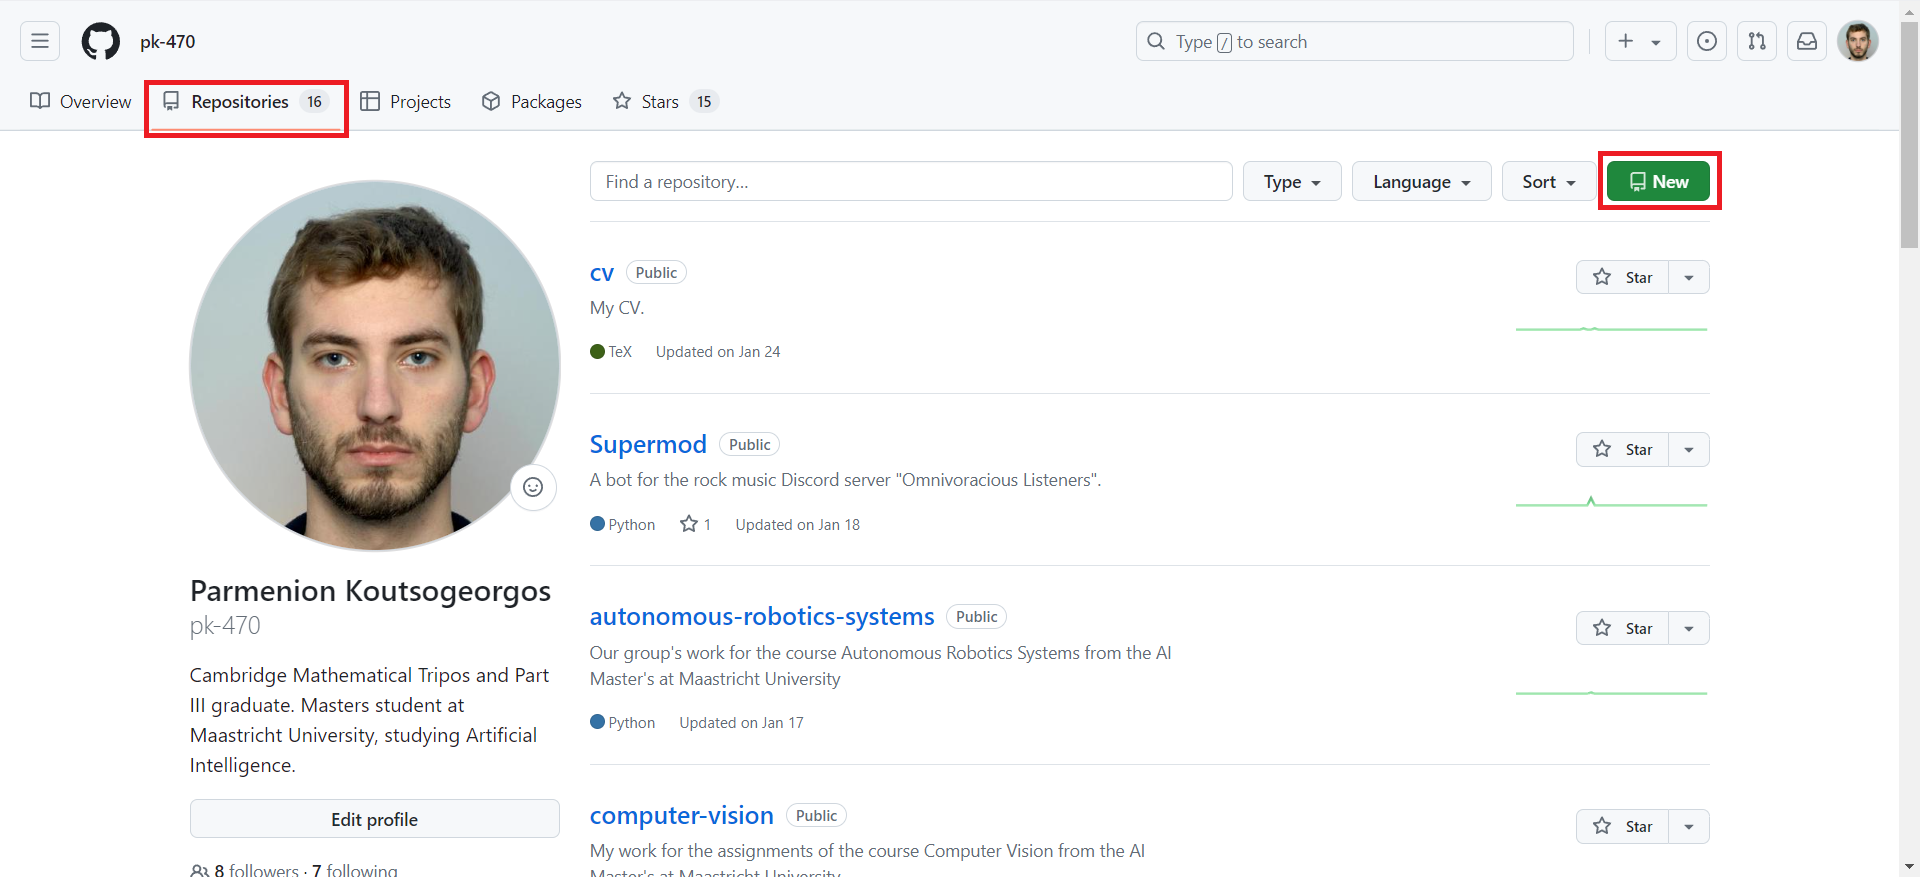
\includegraphics[width=\textwidth]{new_repository.png}
    \caption{Start a new repository.}
    \label{fig:new_repository}   
\end{figure}

A menu as shown in \Cref{fig:new_repository_options} should appear. The following are important:
\begin{enumerate}
    \item Choose yourself as the repository owner.
    \item Write down the local Git repository name as the GitHub repository name.
    \item Make the repository public so that others will not need special permissions to view it, and more importantly so that you can deploy it on GitHub Pages for free. Note that even if the repository is public, nobody else will be able to edit it without permission.
\end{enumerate}
You can also add a short description if you want. No other default options need to be changed. You can click \emph{Create repository} after you are done. You should now be redirected to your new repository, at:

\url{https://github.com/StefanMaubach/mvc-self-learning-module}

\begin{figure}[htbp]
    \centering
    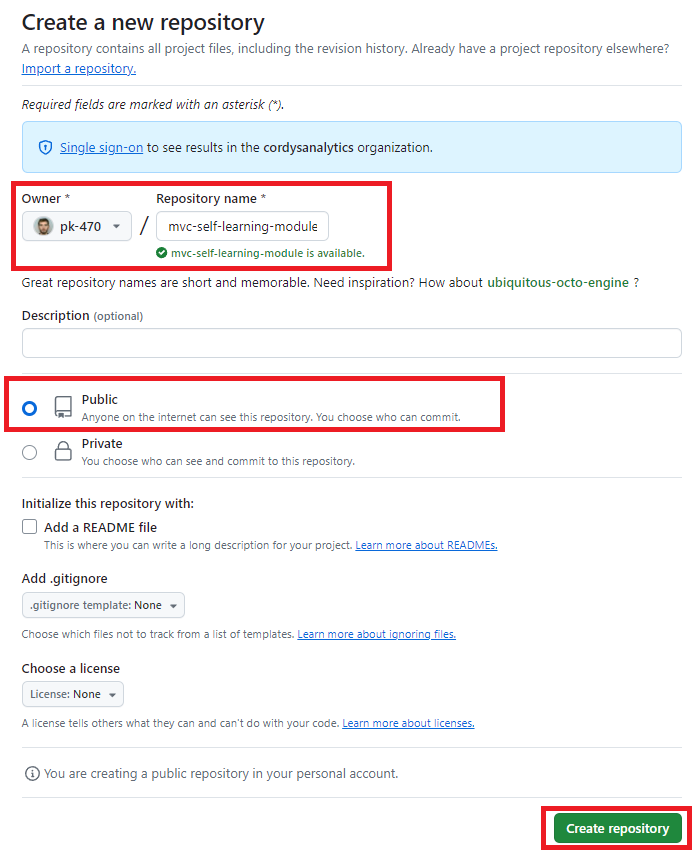
\includegraphics[width=0.75\textwidth]{new_repository_options.png}
    \caption{New repository options.}
    \label{fig:new_repository_options}   
\end{figure}

\paragraph{Associating your local Git repository with an empty GitHub repository.} I assume now that:
\begin{itemize}
    \item You have a local Git repository for your project, preferably (but not necessarily) one at which at least one commit has been made.
    \item You have an empty GitHub repository in which you want to push your local Git repository.
\end{itemize}
If the GitHub repository is indeed still empty, a helpful guide such as in \Cref{fig:new_repository_setup} should appear when you access the repository through a browser. Make sure to select the \emph{HTTPS} option of the guide as the SSH option requires further setup (although nowadays the SSH option is often preferred because of security reasons). Assuming that you already have a local Git repository, simply open its directory in a terminal as before and follow the second block of instructions shown in the guide. A few words about each line:
\begin{enumerate}
    \item The first line:

    \texttt{git remote add origin https://github.com/StefanMaubach/mvc-self-learning-module.git}
    
    is the one that actually associates the local Git repository with the remote GitHub repository.
    
    \item Technically the second line:
    
    \texttt{git branch -M main}
    
    is not needed. It is there because the main Git branch used to be called \emph{master} instead of \emph{main}, so this line is there to simply ensure compatibility with older repositories. If you installed Git using the default options, you do not need this.

    \item The third line:

    \texttt{git push -u origin main}

    is needed ONLY IF YOU HAVE MADE AT LEAST ONE COMMIT TO YOUR LOCAL GIT REPOSITORY. Otherwise this line will throw an error in the terminal (which you can ignore), as there is no commit to push. You may skip this line until you are happy with a version of your website that you want to be up and running. Whenever you want your files to be pushed to GitHub however, so that the website can be deployed, go back to \Cref{sec:first_commit} and make your first commit, and then use this line to push it to the main branch on the remote GitHub repository.
\end{enumerate}
The terminal output should look something like \Cref{fig:git_remote_add_origin}.

\begin{figure}[htbp]
    \centering
    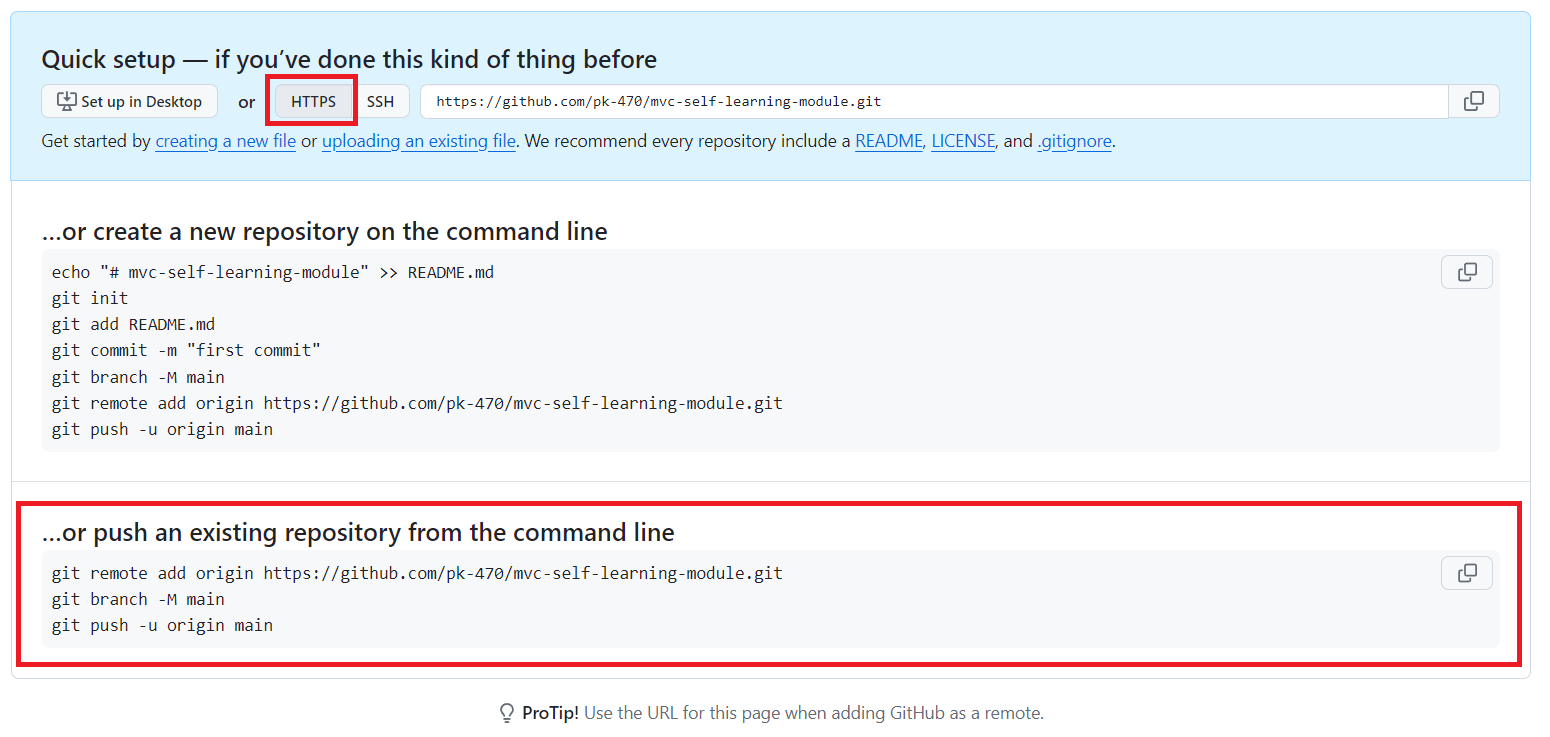
\includegraphics[width=\textwidth]{new_repository_setup.png}
    \caption{New repository setup.}
    \label{fig:new_repository_setup}   
\end{figure}

\begin{figure}[htbp]
    \centering
    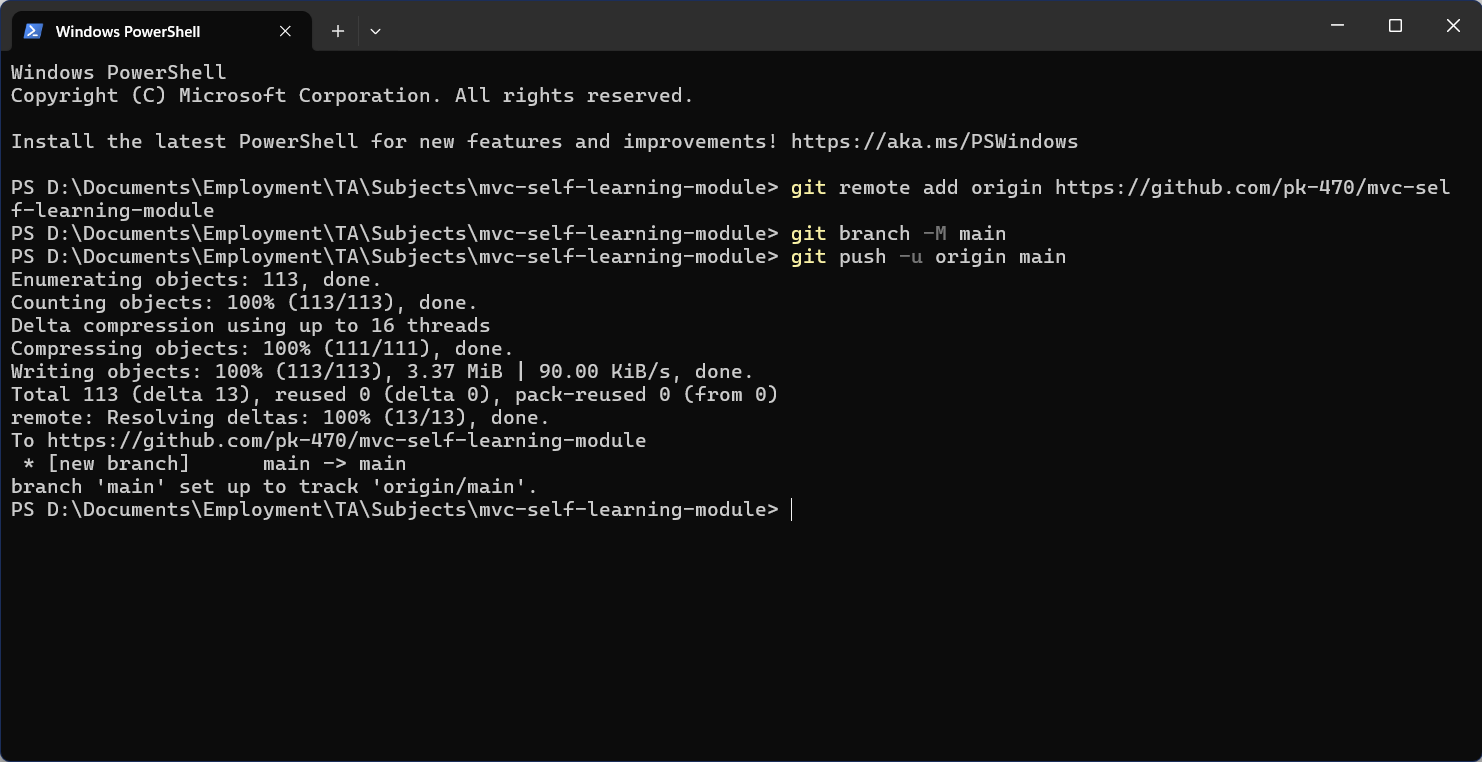
\includegraphics[width=\textwidth]{git_remote_add_origin.png}
    \caption{Associate local Git repository with remote GitHub repository and push the local commits.}
    \label{fig:git_remote_add_origin}   
\end{figure}

\subsection{GitHub Pages}

It is time to deploy the website on GitHub Pages! I now assume that:
\begin{itemize}
    \item You have a local Git repository for your project at which at least one commit has been made.
    \item You have a GitHub repository associated with your local Git repository.
    \item You have pushed your local commits to the remote GitHub repository.
\end{itemize}
If you access the GitHub repository through your browser, it should look something like \Cref{fig:mvc_repository}.

\begin{figure}[htbp]
    \centering
    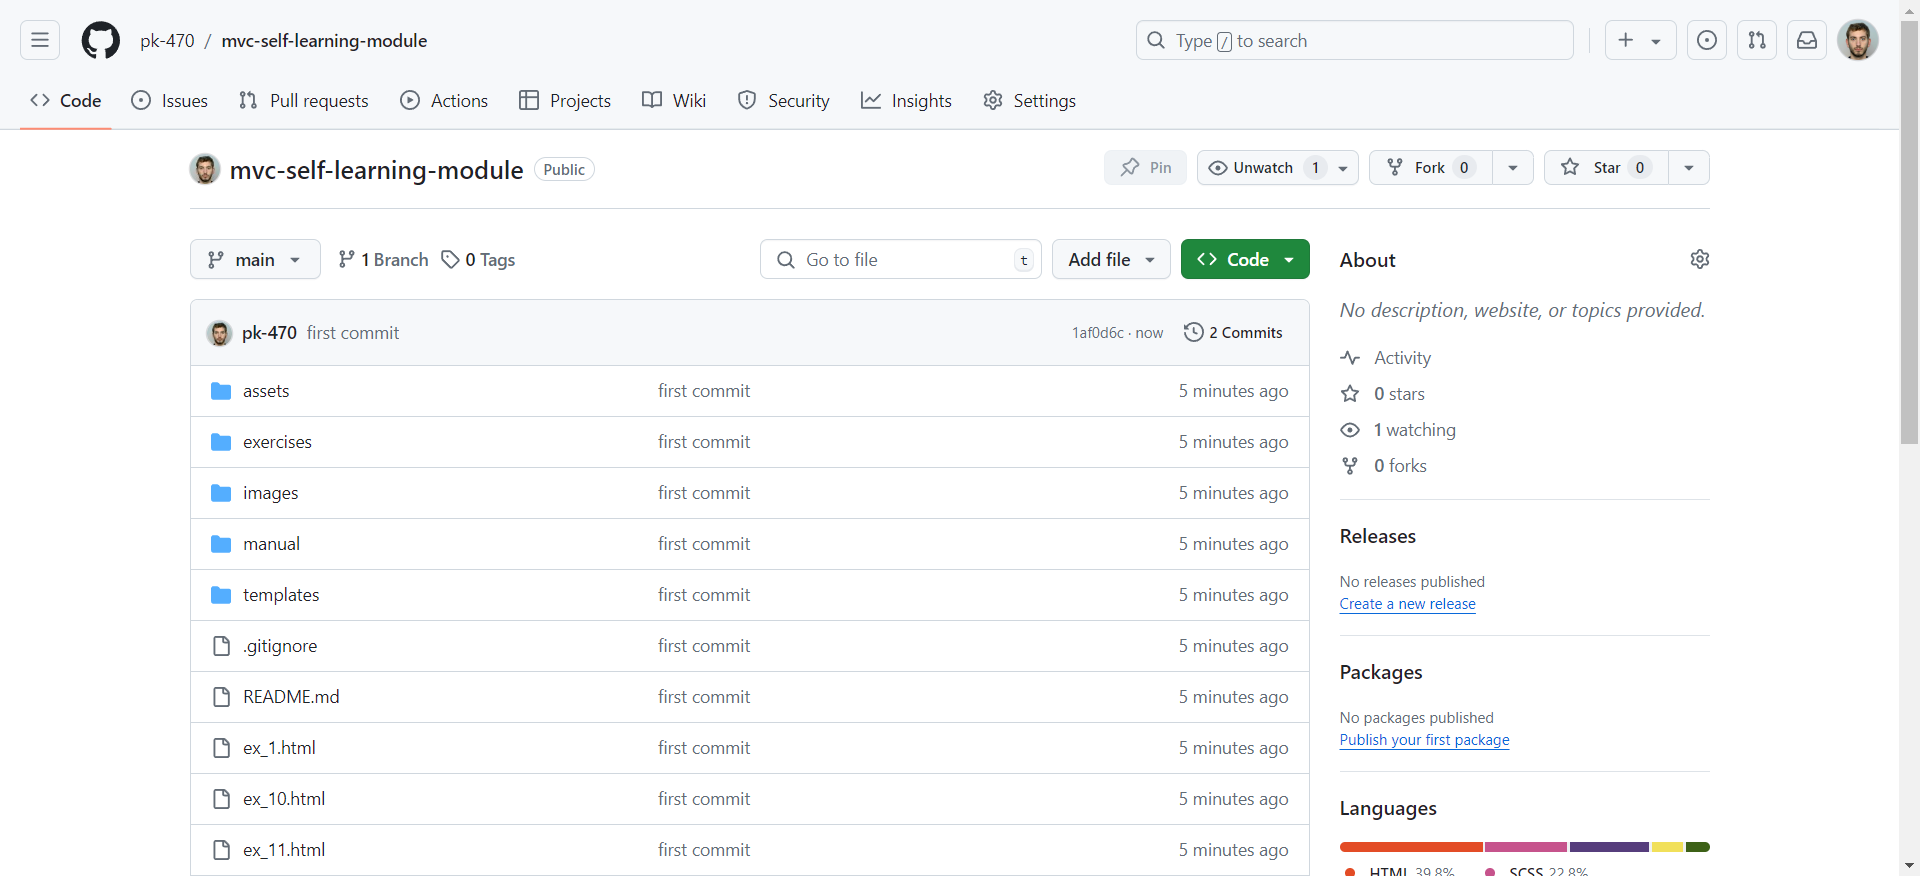
\includegraphics[width=\textwidth]{mvc_repository.png}
    \caption{GitHub repository after setup and first push.}
    \label{fig:mvc_repository}   
\end{figure}

In order to deploy the repository as a website on GitHub pages, go to \emph{Settings} (on the top) $>$ \emph{Pages} (on the left). Then at section \emph{Build and deployment} and subsection \emph{Branch} choose the \emph{main} branch and click \emph{Save} (\Cref{fig:mvc_deploy}).

\begin{figure}[htbp]
    \centering
    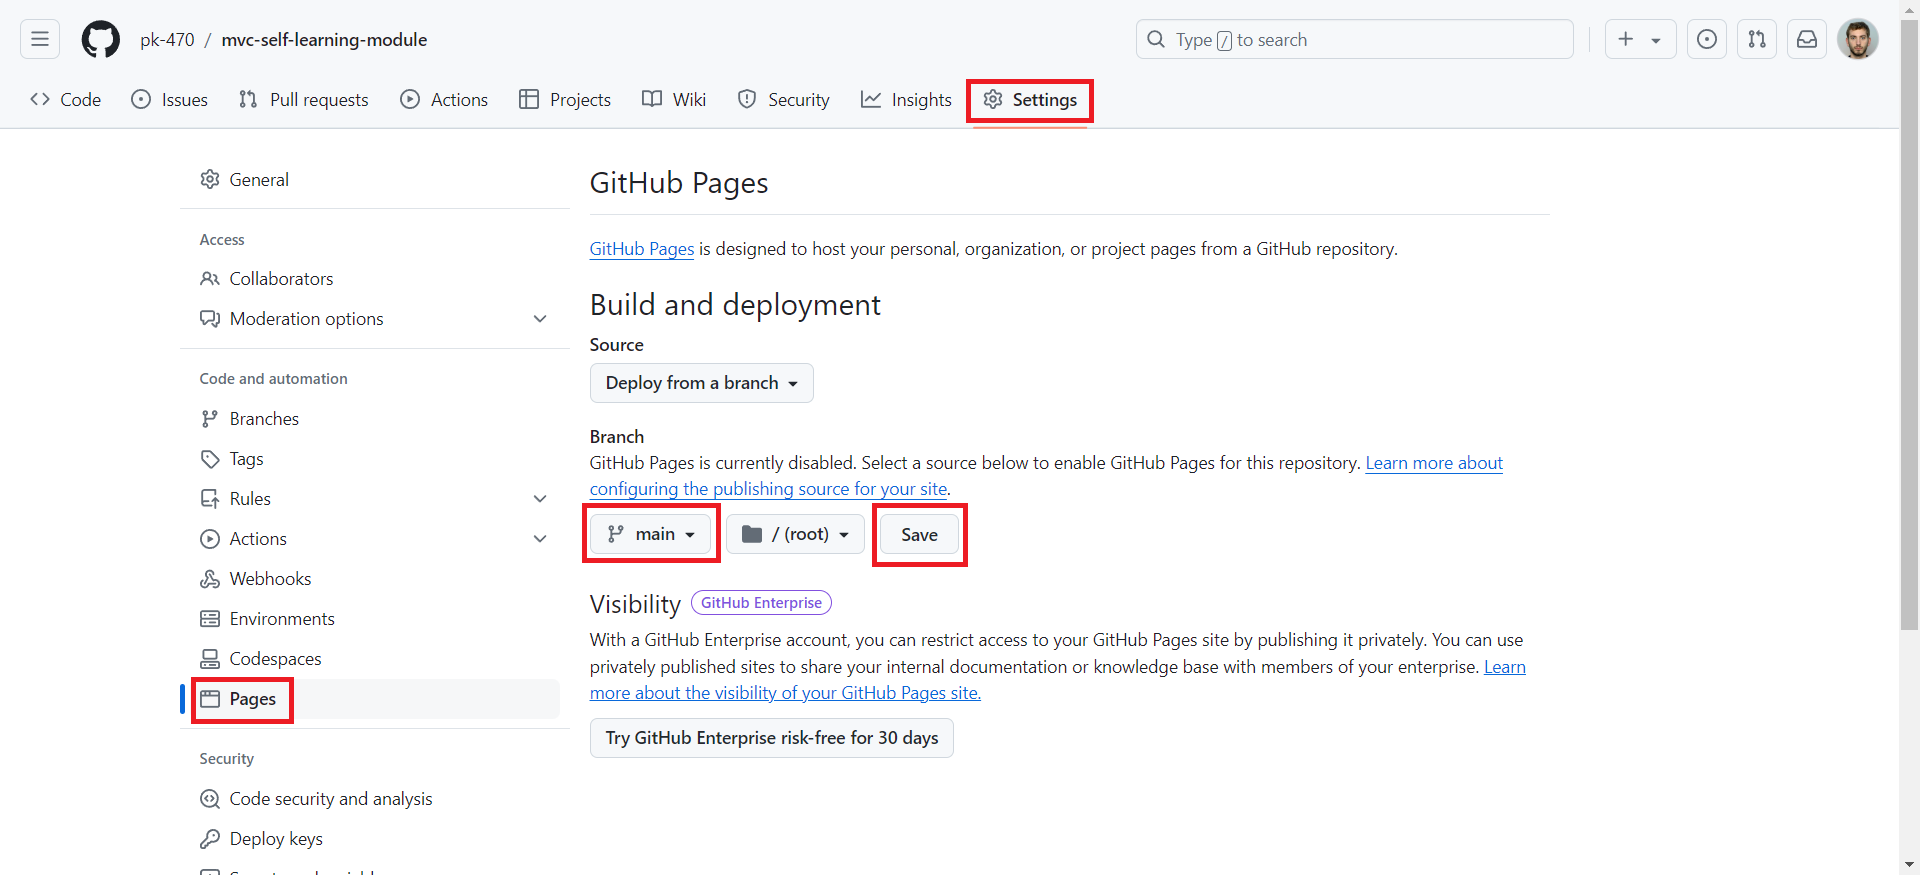
\includegraphics[width=\textwidth]{mvc_deploy.png}
    \caption{Deploy the repository on GitHub Pages.}
    \label{fig:mvc_deploy}   
\end{figure}

\subsubsection{Link to the website}

If you go back to your main GitHub repository page after deployment, you should see a new section named \emph{Deployments} on the right sidebar (\Cref{fig:mvc_deployment_added}).

\begin{figure}[htbp]
    \centering
    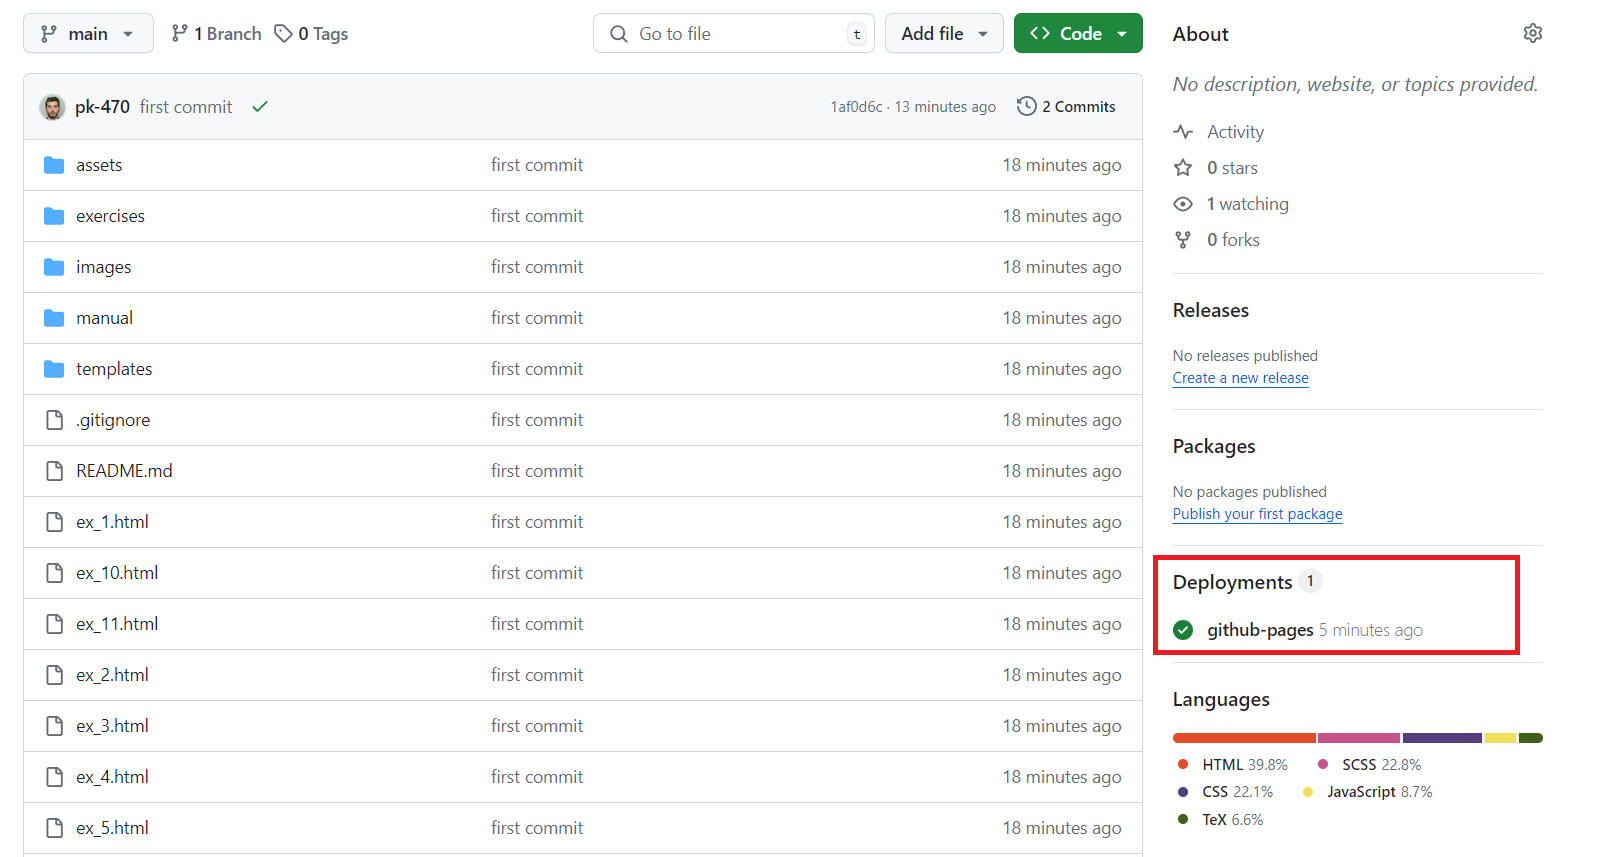
\includegraphics[width=\textwidth]{mvc_deployment_added.png}
    \caption{Deployment section added to the sidebar of the repository.}
    \label{fig:mvc_deployment_added}   
\end{figure}

Clicking on \emph{github-pages} should lead to a page similar to \Cref{fig:deployment}.

\begin{figure}[htbp]
    \centering
    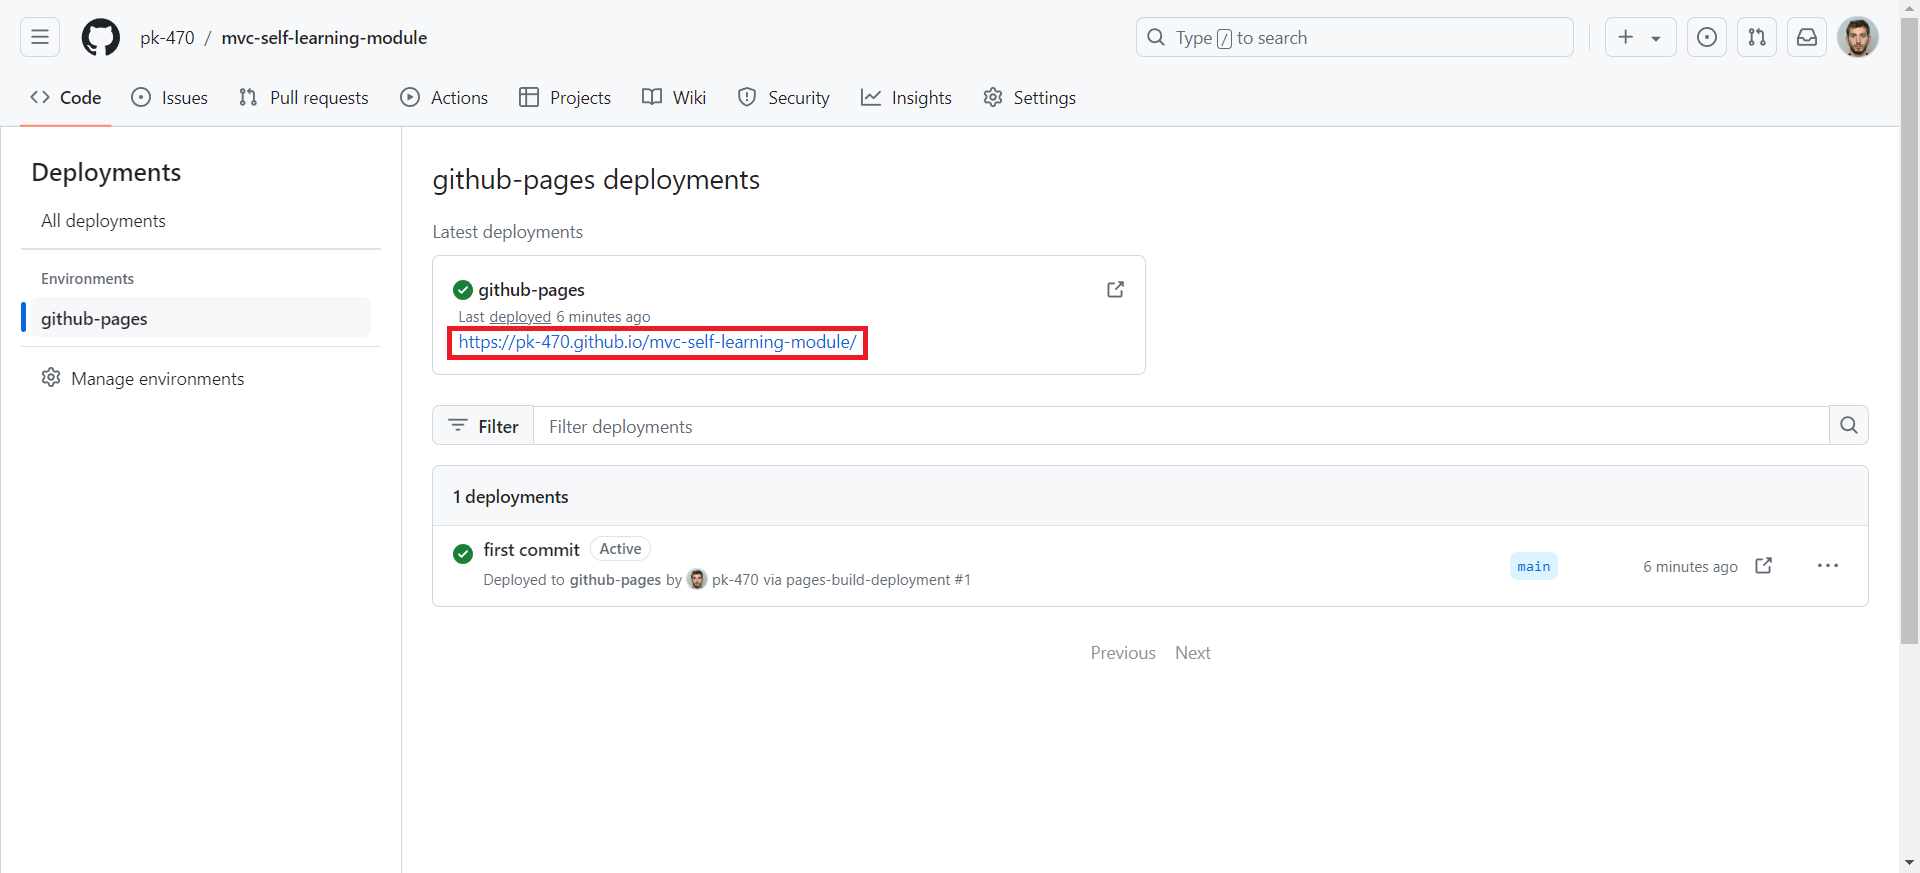
\includegraphics[width=\textwidth]{deployment.png}
    \caption{Deployment page for the repository.}
    \label{fig:deployment}   
\end{figure}

Finally, following the first link should lead to the website (\Cref{fig:website}). The website will remain in this link (unless you decide to change the domain, which can be done but is more complicated), and will update itself whenever you make a new commit and push it to the GitHub repository.

\begin{figure}[htbp]
    \centering
    
\includegraphics[width=\textwidth]{website.png}
    \caption{Deployed live website.}
    \label{fig:website}   
\end{figure}


\subsection{VSCode (optional)}
\label{sec:vscode}

I recommend using Visual Studio Code (VSCode) to edit HTML or any other files that you don't already know how to edit easily. VSCode is a free and lightweight text editor that can be customised to work with almost every programming or markup language (including \LaTeX) using extensions. You can download VSCode from:

\url{https://code.visualstudio.com/}

The default installation options are fine.

In order to add extensions to VSCode, you need to click on the block-looking icon on the left sidebar. This should open a small window next to the left sidebar, which is titled \emph{Extensions} and contains (e.g.\ \Cref{fig:extensions}):
\begin{itemize}
    \item a search bar;
    \item a list with your installed extensions;
    \item possibly, some recommended extensions.
\end{itemize}

\begin{figure}[htbp]
    \centering
    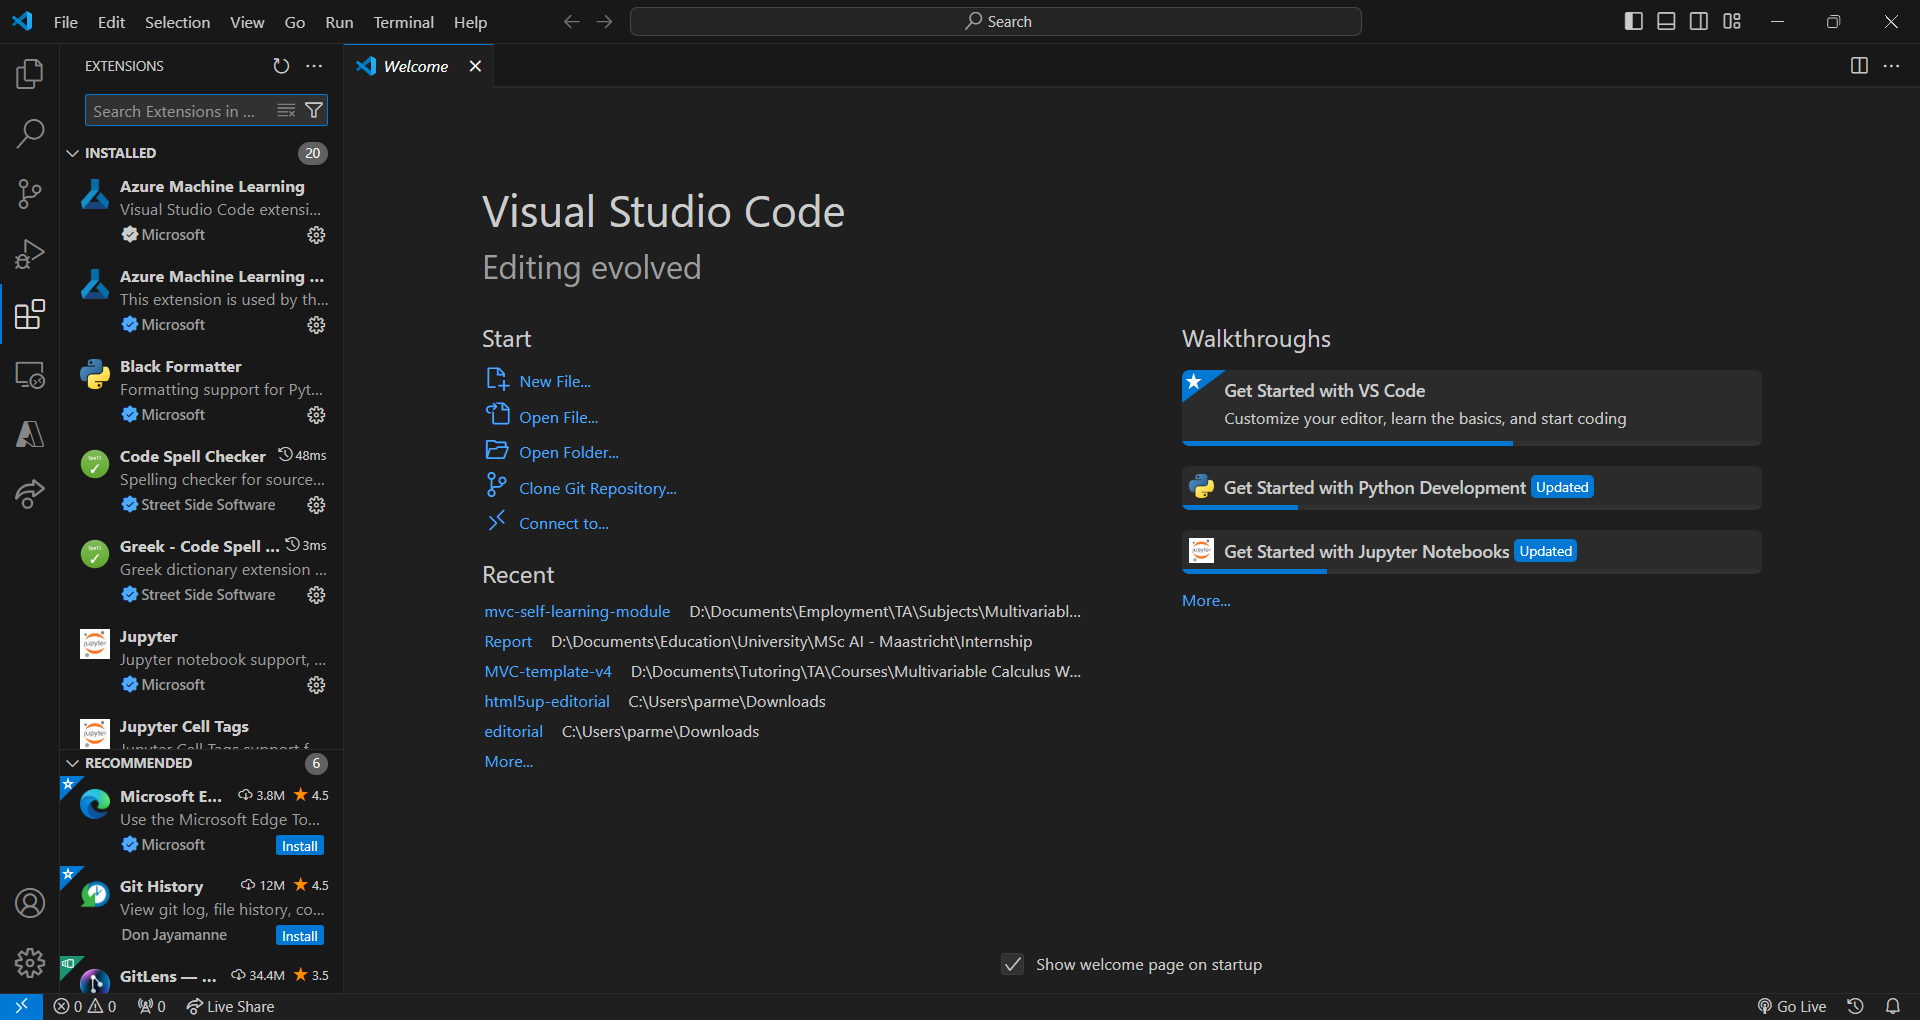
\includegraphics[width=\textwidth]{extensions.png}
    \caption{VSCode extensions.}
    \label{fig:extensions}   
\end{figure}

You can use the search bar to search for new extensions to install. For the purposes of this project I recommend the following two extensions:

\paragraph{Live Server.} This extension is used to produce a local live server so that you can run and directly see the changes you make while editing the website. It is also useful because some JavaScript components will not run when you view the website through the Windows file system, i.e.\ when the path on your browser looks like \emph{C://\dots} instead of \emph{http://\dots} or \emph{https://\dots}. You can install \emph{Live Server} as shown in \Cref{fig:live_server}. If you have not already installed the extension, there should be an \emph{Install} option around where \emph{Uninstall} is in the picture.

\begin{figure}[htbp]
    \centering
    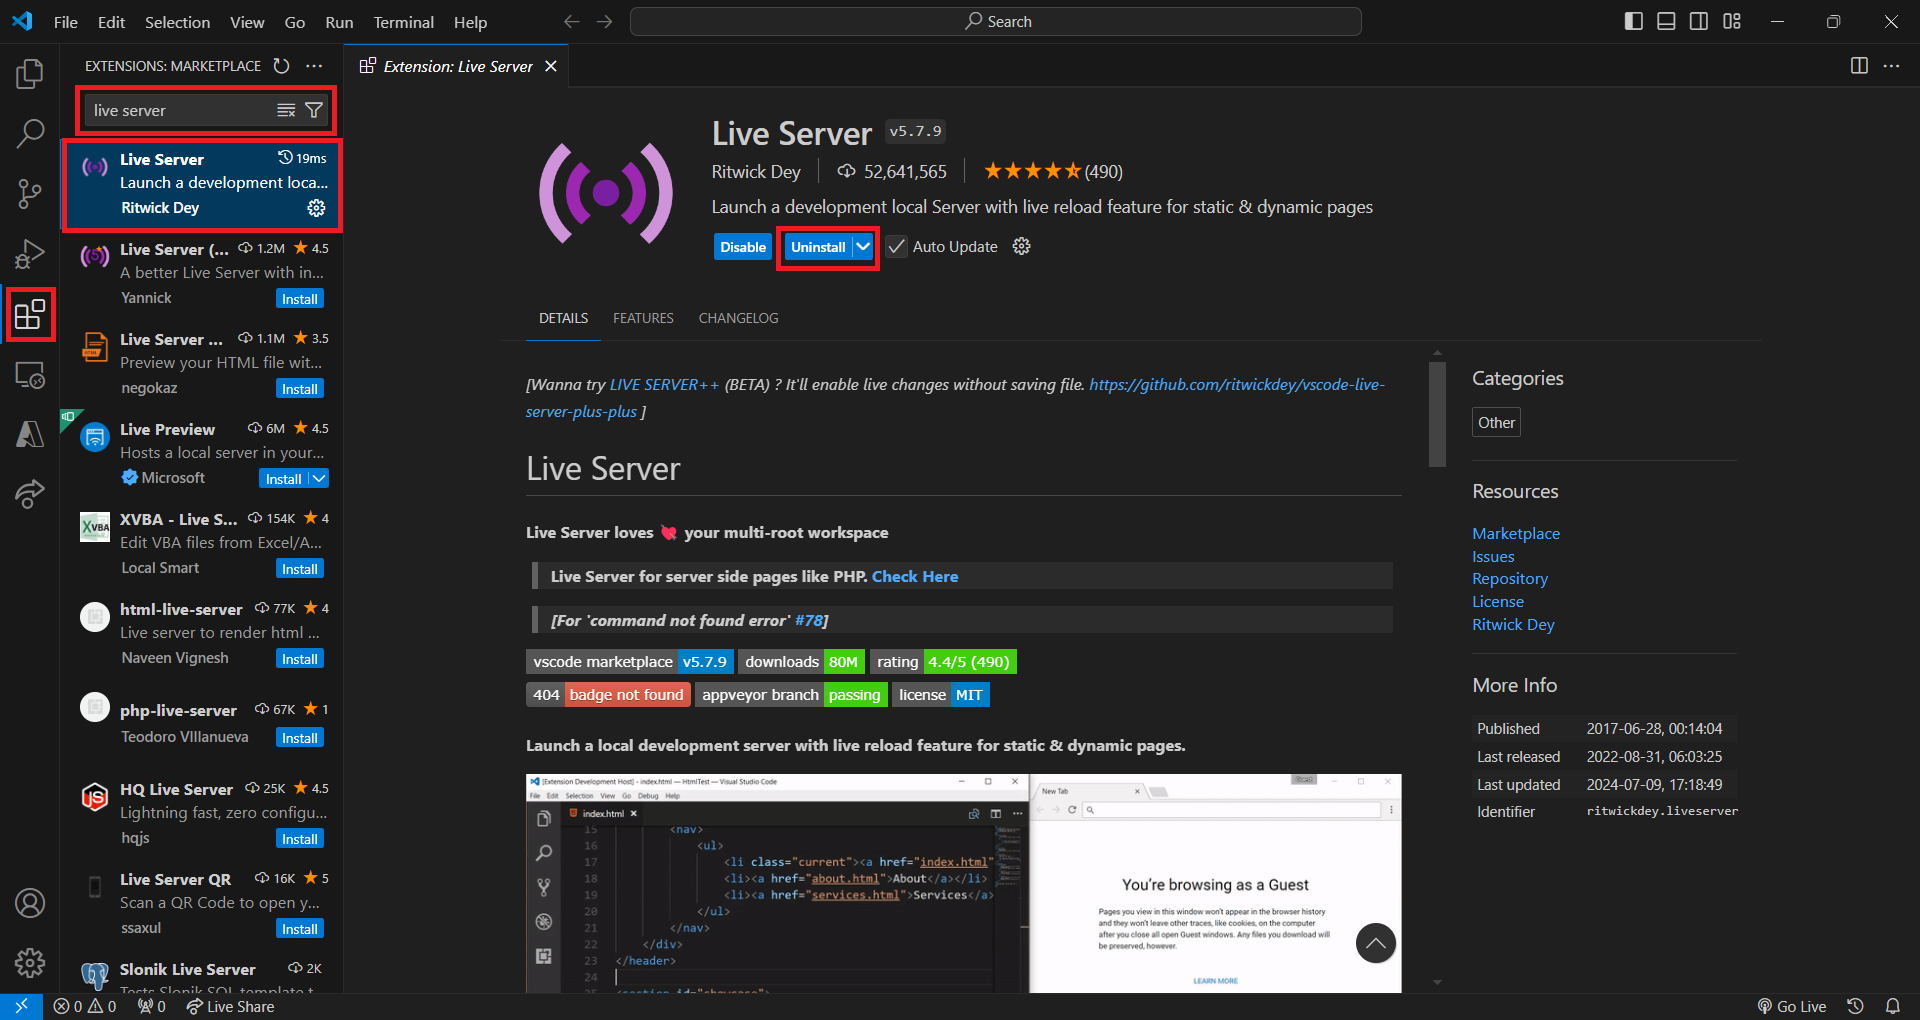
\includegraphics[width=\textwidth]{live_server.png}
    \caption{\emph{Live Server} extension.}
    \label{fig:live_server}   
\end{figure}

\paragraph{Prettier.} This extension is used to format code in a way that makes it easier to read, which makes bugs easier to see, which has been proven to significantly increase life expectancy over time. You can install \emph{Prettier} as shown in \Cref{fig:prettier}. If you have not already installed the extension, there should be an \emph{Install} option around where \emph{Uninstall} is in the picture.

\begin{figure}[htbp]
    \centering
    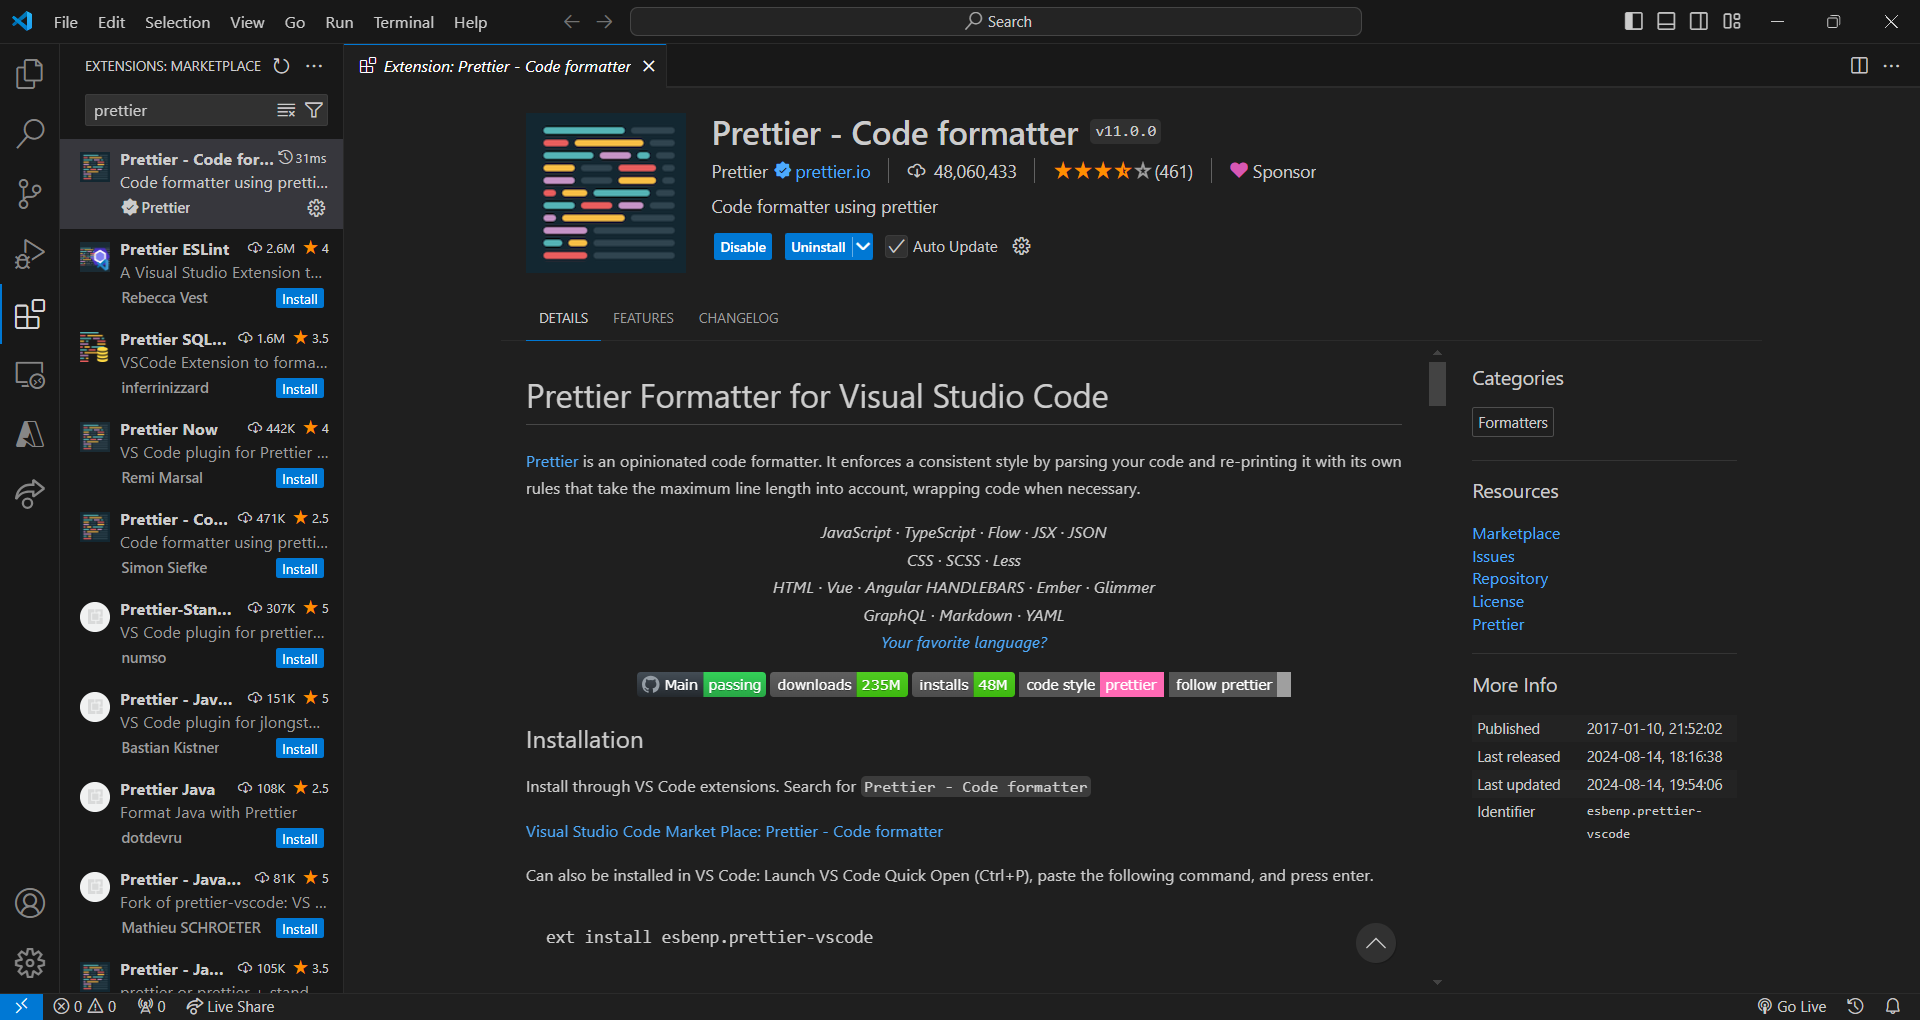
\includegraphics[width=\textwidth]{prettier.png}
    \caption{\emph{Prettier} extension.}
    \label{fig:prettier}   
\end{figure}

\subsection{Python (optional)}

In order to use the Python script, you need to have a local installation of Python. You can download the latest version of Python from:

\url{https://www.python.org/downloads/}

The website should recommend the latest installer for Windows. During the installation process, MAKE SURE TO CHECK THE BOX THAT ADDS PYTHON TO PATH! Otherwise, you will have to do it manually in order to run Python scripts. In order to do it manually, Google something like ``add python to path'' followed by your system, and follow the detailed instructions.

\clearpage
\section{Usage}

Finally, everything is set up! You should now have:
\begin{itemize}
    \item a local Git repository for your project at which at least one commit has been made;
    \item a GitHub repository which is up to date with your local Git repository;
    \item an up and running website deployed on GitHub Pages from your GitHub repository.
\end{itemize}
From now on, things should be much easier! 

\subsection{Updating the website}

In order to work with the update pipeline (Git $\to$ GitHub $\to$ GitHub Pages), you only need the following steps: 
\begin{enumerate}
    \item Pull any changes made to the repository from someone else. This should be done IF AND ONLY IF THERE ARE MULTIPLE COMPUTERS WORKING ON THE SAME BRANCH. Otherwise, Git may find conflicts between the changes made in each computer's local commits and those in the global repository, and you may need to enter the super annoying process of merging conflicts, i.e.\ telling Git what to keep from each commit. If you are only working on the branch on a single computer yourself, feel free to skip this step. If you need to perform it however (e.g.\ if you work on the repository from multiple computers, or if you get another TA to work on this and they don't use a separate branch), use the command:

    \texttt{git pull origin main}

    IMPORTANT NOTE: After setup is complete, always use \texttt{git pull} and never \texttt{git clone}. Otherwise you will clone the repository as it is on GitHub again, and you will lose any local changes!  

    \item From now on, you simply make your changes, and commit in the exact same way as the first commit. For example, I made some changes in this manual. I will commit them as follows:

    \texttt{get add .}

    \texttt{git commit -m "manual ctd"}

    \item Finally, push the changes to the GitHub repository. Just like in the first push, you can do this as follows:

    \texttt{git push origin main}
\end{enumerate}
A couple of notes:
\begin{itemize}
    \item During the first or third steps above, Git may require from you to verify your identity by opening a popup window and asking for your GitHub credentials. Simply login as it says, and ignore or close any extra browser windows that may appear.
    \item If you included the \texttt{-u} flag in the first \texttt{git push}, technically you can use \texttt{git pull} and \texttt{git push} without any arguments. However, I think consistency and clarity makes things easier.
\end{itemize}

That's it! GitHub Pages will now see the new changes from your GitHub repository and it will automatically deploy the new version of the website along with the latest edits. 

If you are using VSCode to edit your files, you can even open the working directory in a terminal within VSCode as shown in \Cref{fig:vscode_open_terminal} and type the above commands there. The output should look something like \Cref{fig:usage}.

\begin{figure}[htbp]
    \centering
    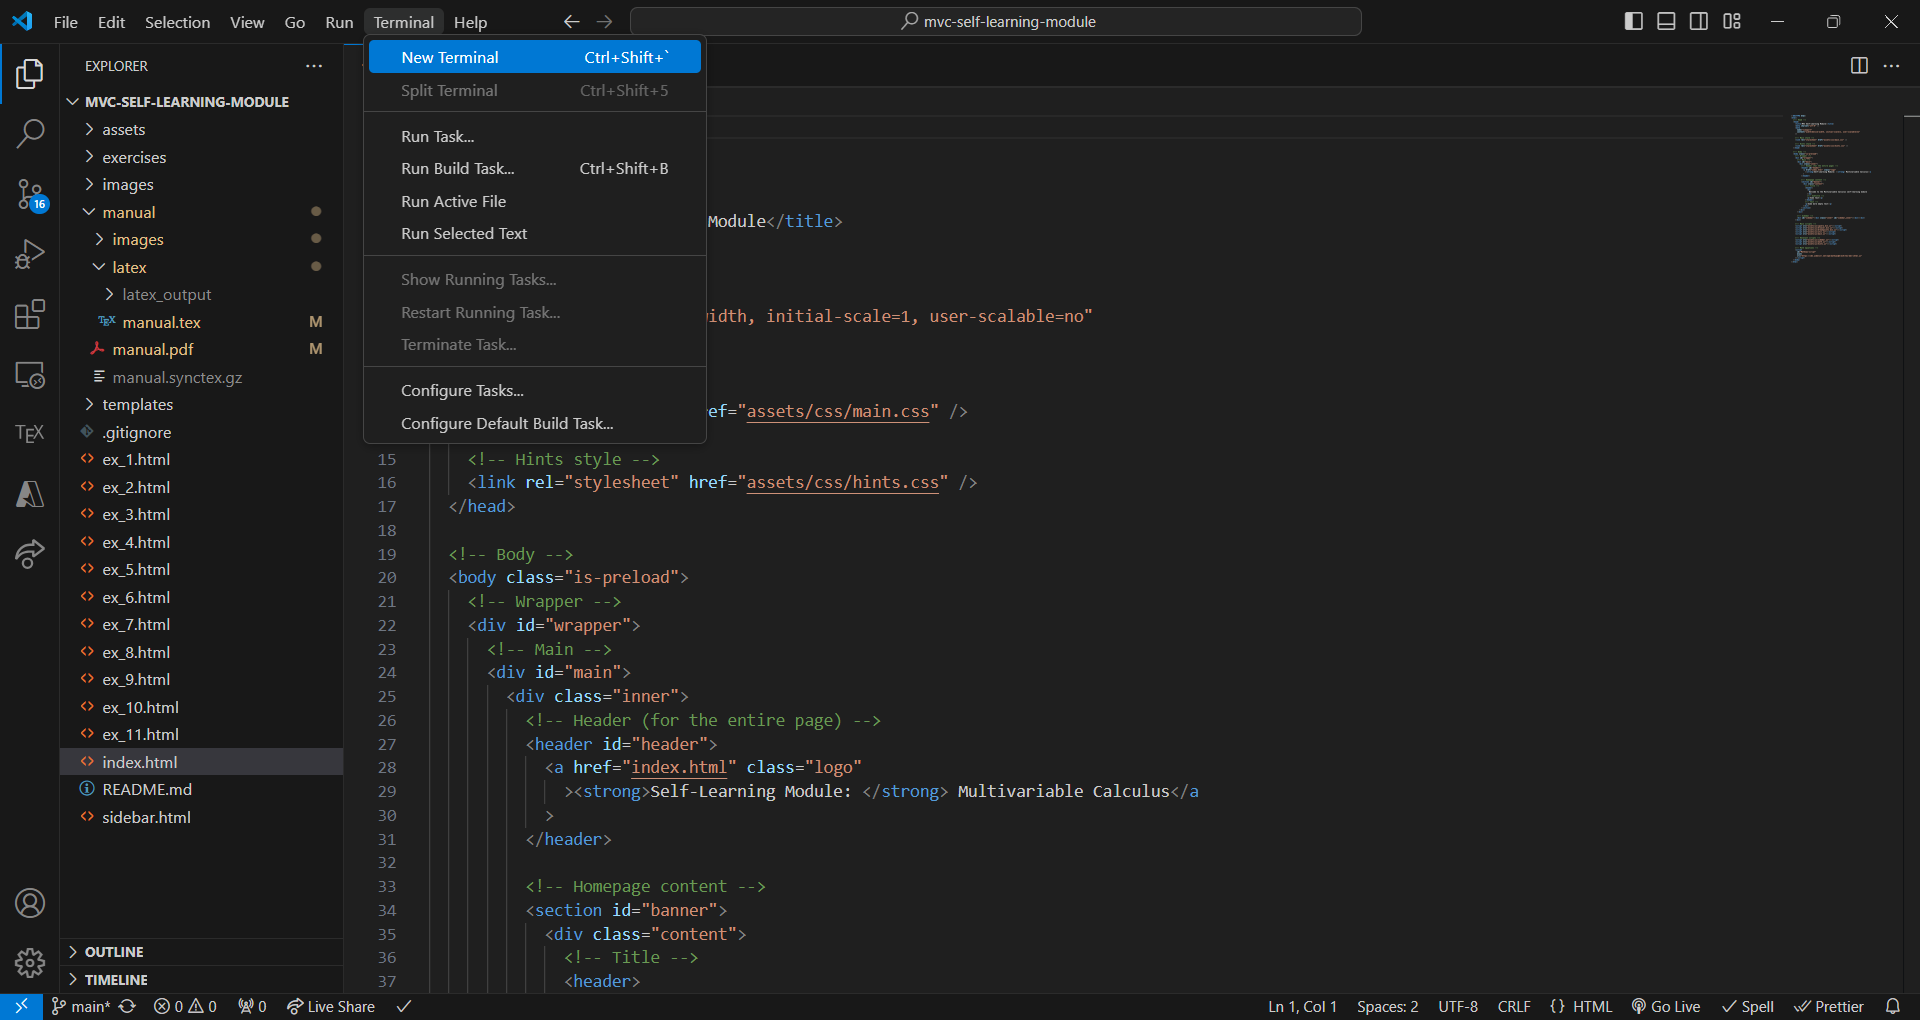
\includegraphics[width=\textwidth]{vscode_open_terminal.png}
    \caption{Open a terminal in VSCode.}
    \label{fig:vscode_open_terminal}   
\end{figure}

\begin{figure}[htbp]
    \centering
    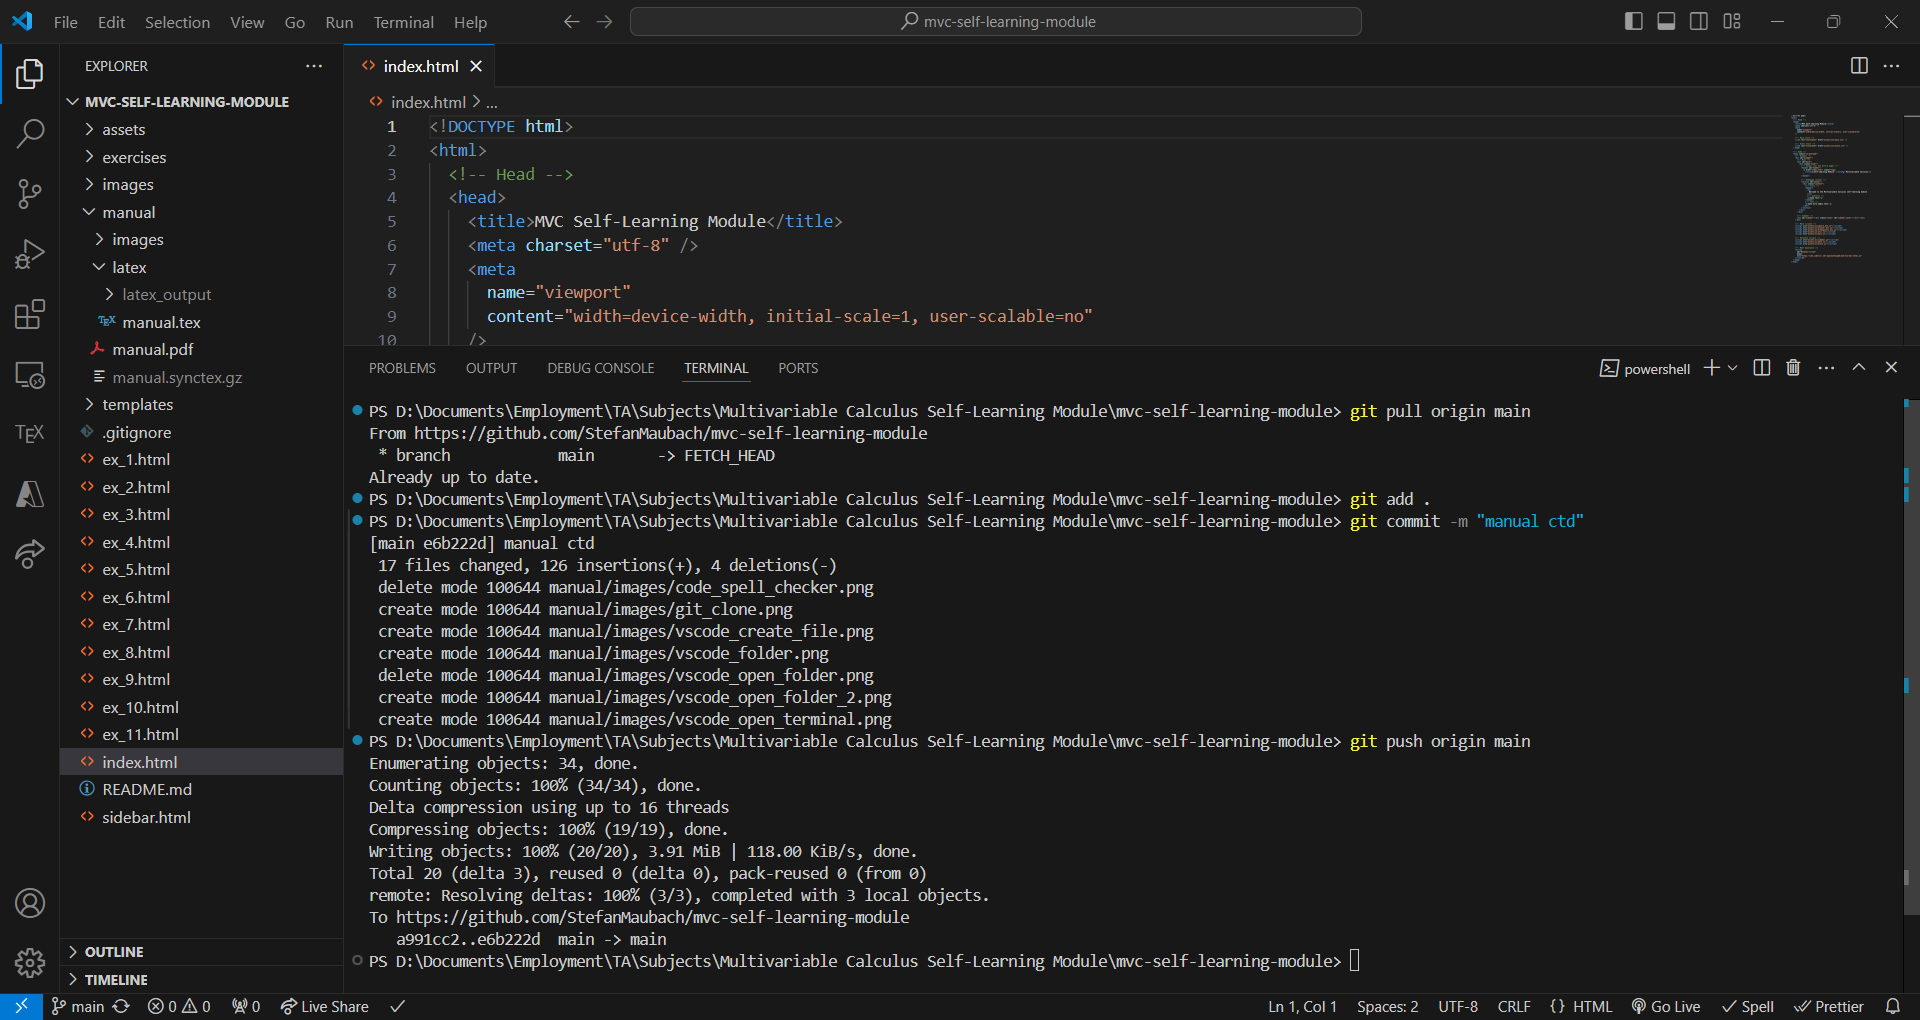
\includegraphics[width=\textwidth]{usage.png}
    \caption{Working with Git from a terminal in VSCode.}
    \label{fig:usage}   
\end{figure}

\subsubsection{Using the Python script to convert \LaTeX\ to HTML (optional)}

If you want, you can add the exercises in a \LaTeX\ document and use the provided script to convert them into individual HTML files. The script should be able to deal with most basic \LaTeX\ environments, including:
\begin{itemize}
    \item figures;
    \item enumerate or itemize environments;
    \item emph, italics, bold or underlined text (up to 3 levels of nesting for these).
\end{itemize}

\paragraph{Writing the exercises in \LaTeX.} In order for the script to work:
\begin{itemize}
    \item Mark clearly each exercise by:
    \begin{verbatim}    \section{Exercise #}\end{verbatim}
    Replace \# by the exercise number.

    \item Write the question right under the section indicator, without marking it by any subsection/paragraph indicators.

    \item Mark clearly each hint by:
    \begin{verbatim}    \subsection{Hint name}\end{verbatim}
    ``Hint name'' is what will show up as a label on the hint button when that appears.
\end{itemize} 
See the \emph{exercises.tex} file (from the root folder it should be located in \emph{./exercises/latex/exercises.tex}) for examples.

\paragraph{Running the Python script.} The Python script is named \emph{tex\_to\_html.py}. You can run the script from a terminal that is open in the same folder as the script (can also be on VSCode) using the command 

\texttt{py tex\_to\_html.py} 

followed by the numbers of the exercises you want to convert, starting from 1. These can be:
\begin{enumerate}
    \item a single number (e.g. 1);
    \item a list of numbers separated by comma (with no spaces) (e.g. 1,2,3);
    \item the word 'all' (without '') if you want to convert all the exercises in the document.
\end{enumerate}

The default path for the \LaTeX\ document is \emph{./exercises/latex/exercises.tex}. You can alter this path when running the script by using the

\texttt{--tex\_path}

flag, followed by the alternative path of the \LaTeX\ document. You can also view and edit all default paths used by the script from the \emph{paths.json} file. You can see all the options provided by the script by running the command

\texttt{py tex\_to\_html.py -h}

Examples of the usage of the Python script can be seen in \Cref{fig:tex_to_html}.

\begin{figure}[htbp]
    \centering
    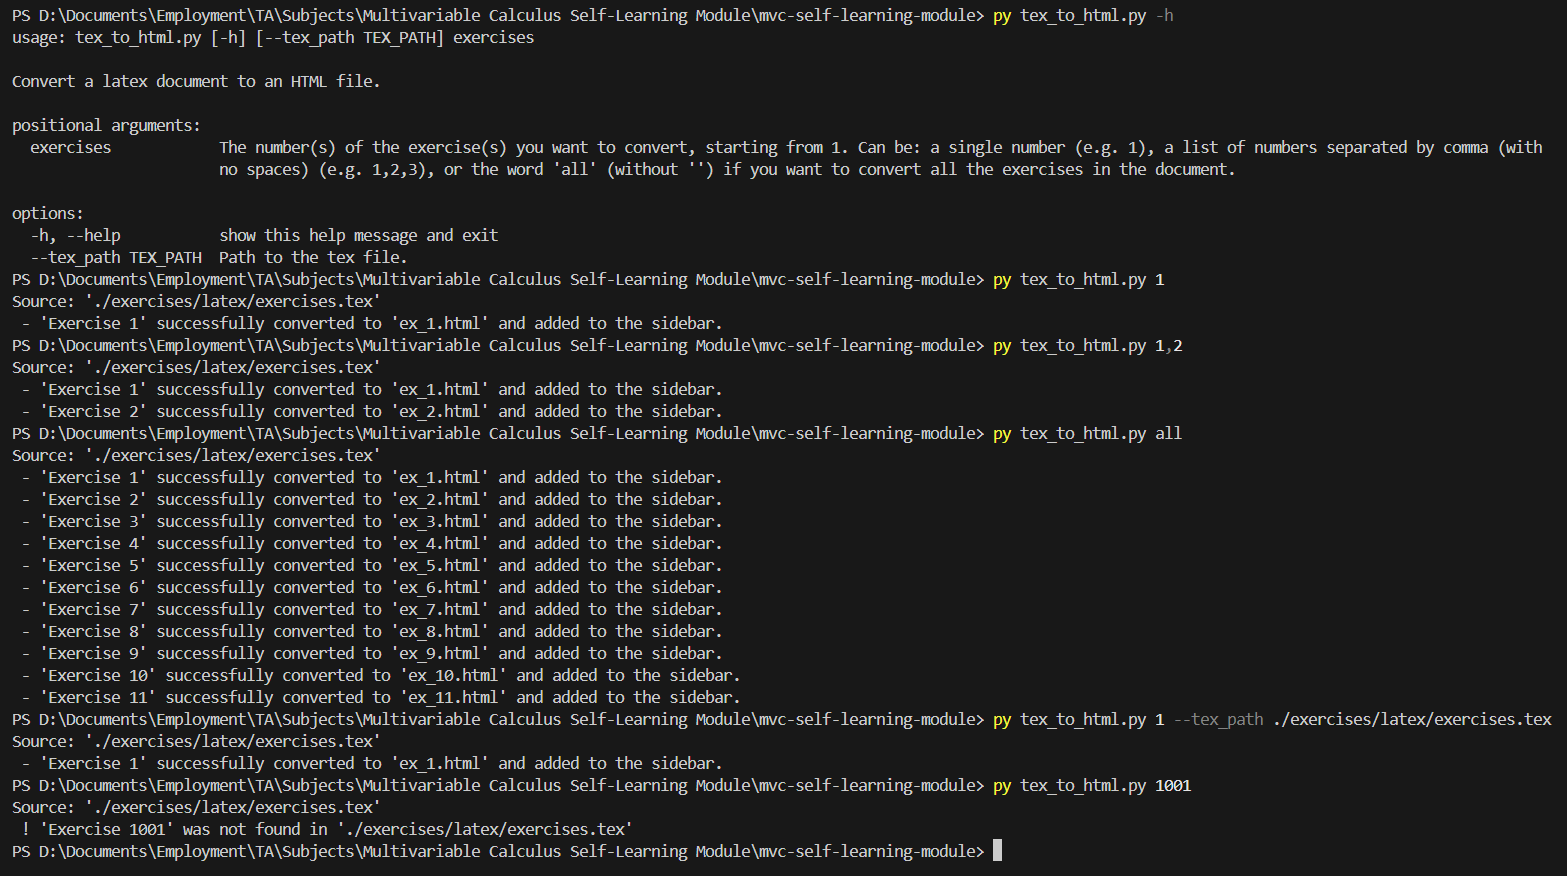
\includegraphics[width=\textwidth]{tex_to_html.png}
    \caption{Example usage of the Python script \emph{tex\_to\_html.py}.}
    \label{fig:tex_to_html}   
\end{figure}


\subsection{Working with VSCode (optional)}

Here are some general instructions about working with VSCode.

\subsubsection{Open a folder in VSCode}

There are multiple ways to open a folder in VSCode. If you have opened a new window without any open folders in it, you can:
\begin{itemize}
    \item Choose the \emph{Open Folder} option from the main window, and search for your folder through the popup File Explorer.
    \item Click on the file-looking icon on the left sidebar, choose the \emph{Open Folder} option from the \emph{Explorer} window that appears on the left, and search for your folder through the popup File Explorer.
    \item if you have opened the desired folder before, you may be able to see your folder in the \emph{Recent} section of the main window and open it directly.
\end{itemize}
All of these options are highlighted in \cref{fig:vscode_open_folder_1}.

\begin{figure}[htbp]
    \centering
    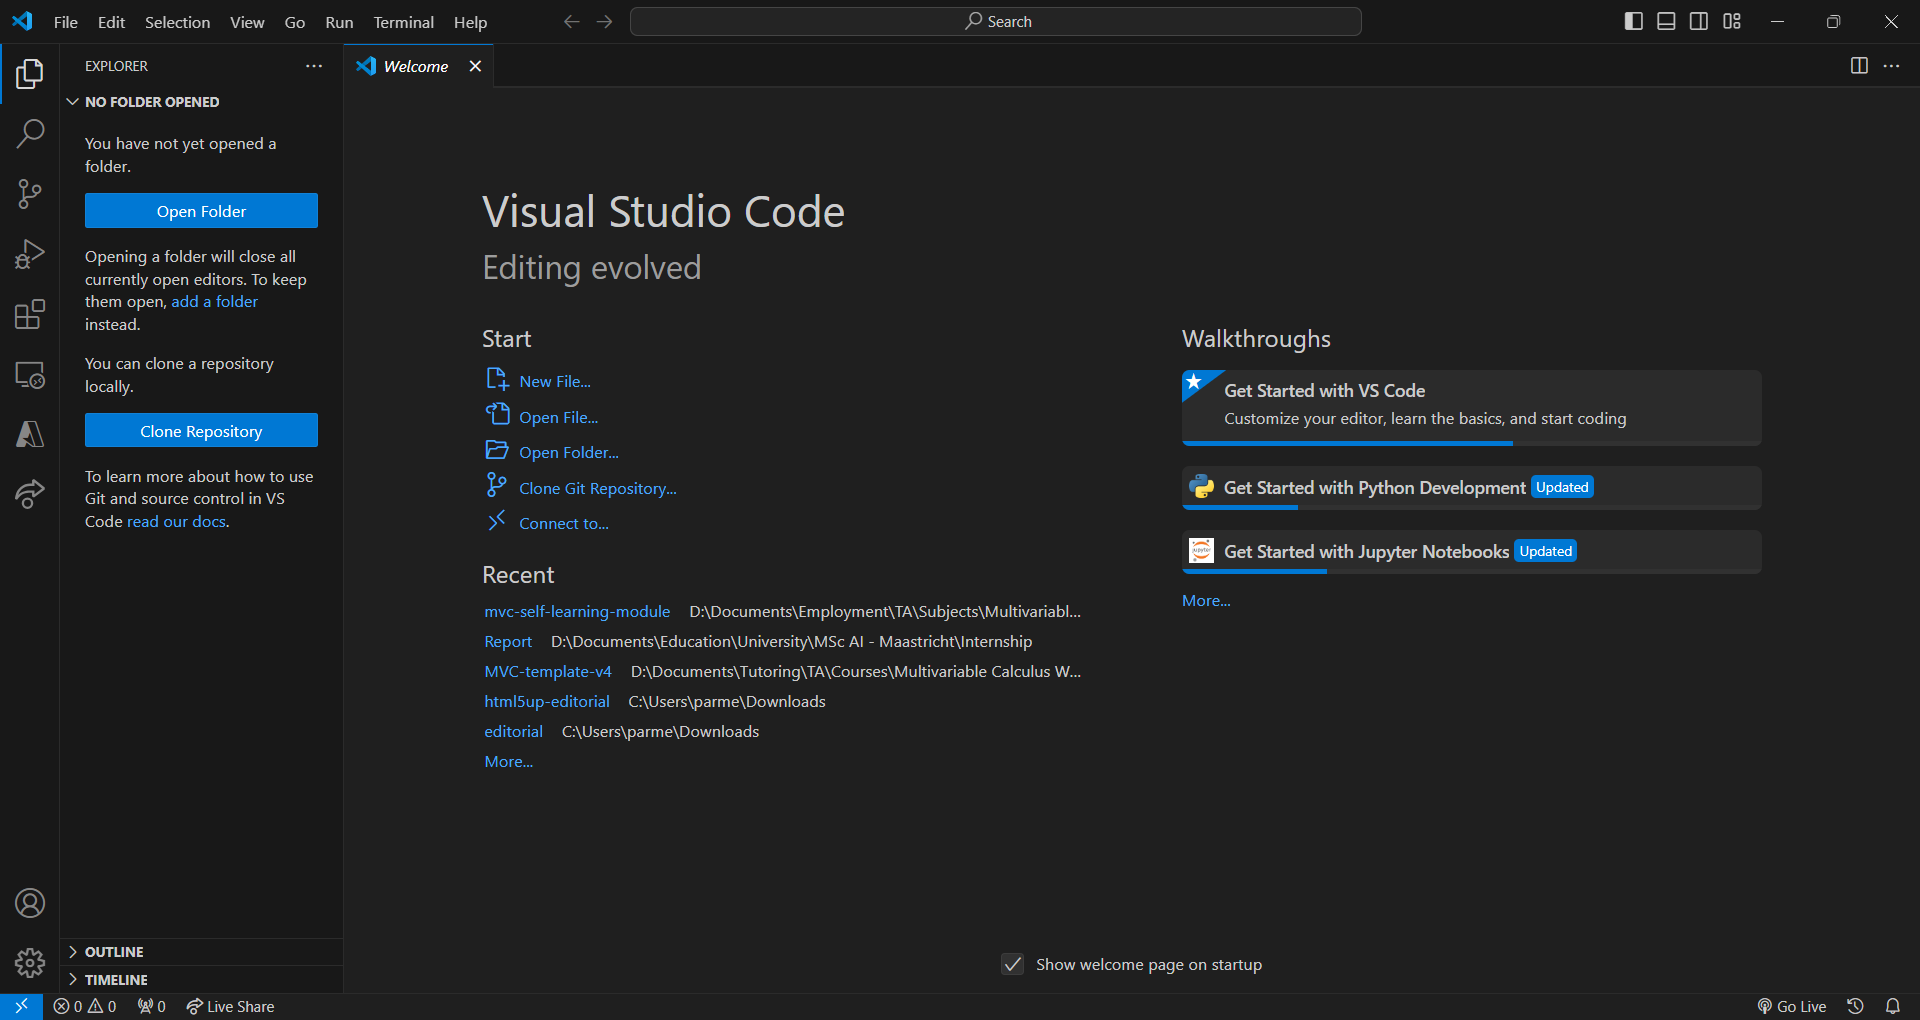
\includegraphics[width=\textwidth]{vscode_open_folder_1.png}
    \caption{Open a folder in an empty window in VSCode.}
    \label{fig:vscode_open_folder_1}   
\end{figure}

If you already have a folder open and you want to open another folder in a new window, you can click on \emph{File} on the top menu, choose \emph{New Window} from the dropdown menu, and choose any of the previous options in the new empty window that will appear (e.g.\ \Cref{fig:vscode_open_folder_2}).

\begin{figure}[htbp]
    \centering
    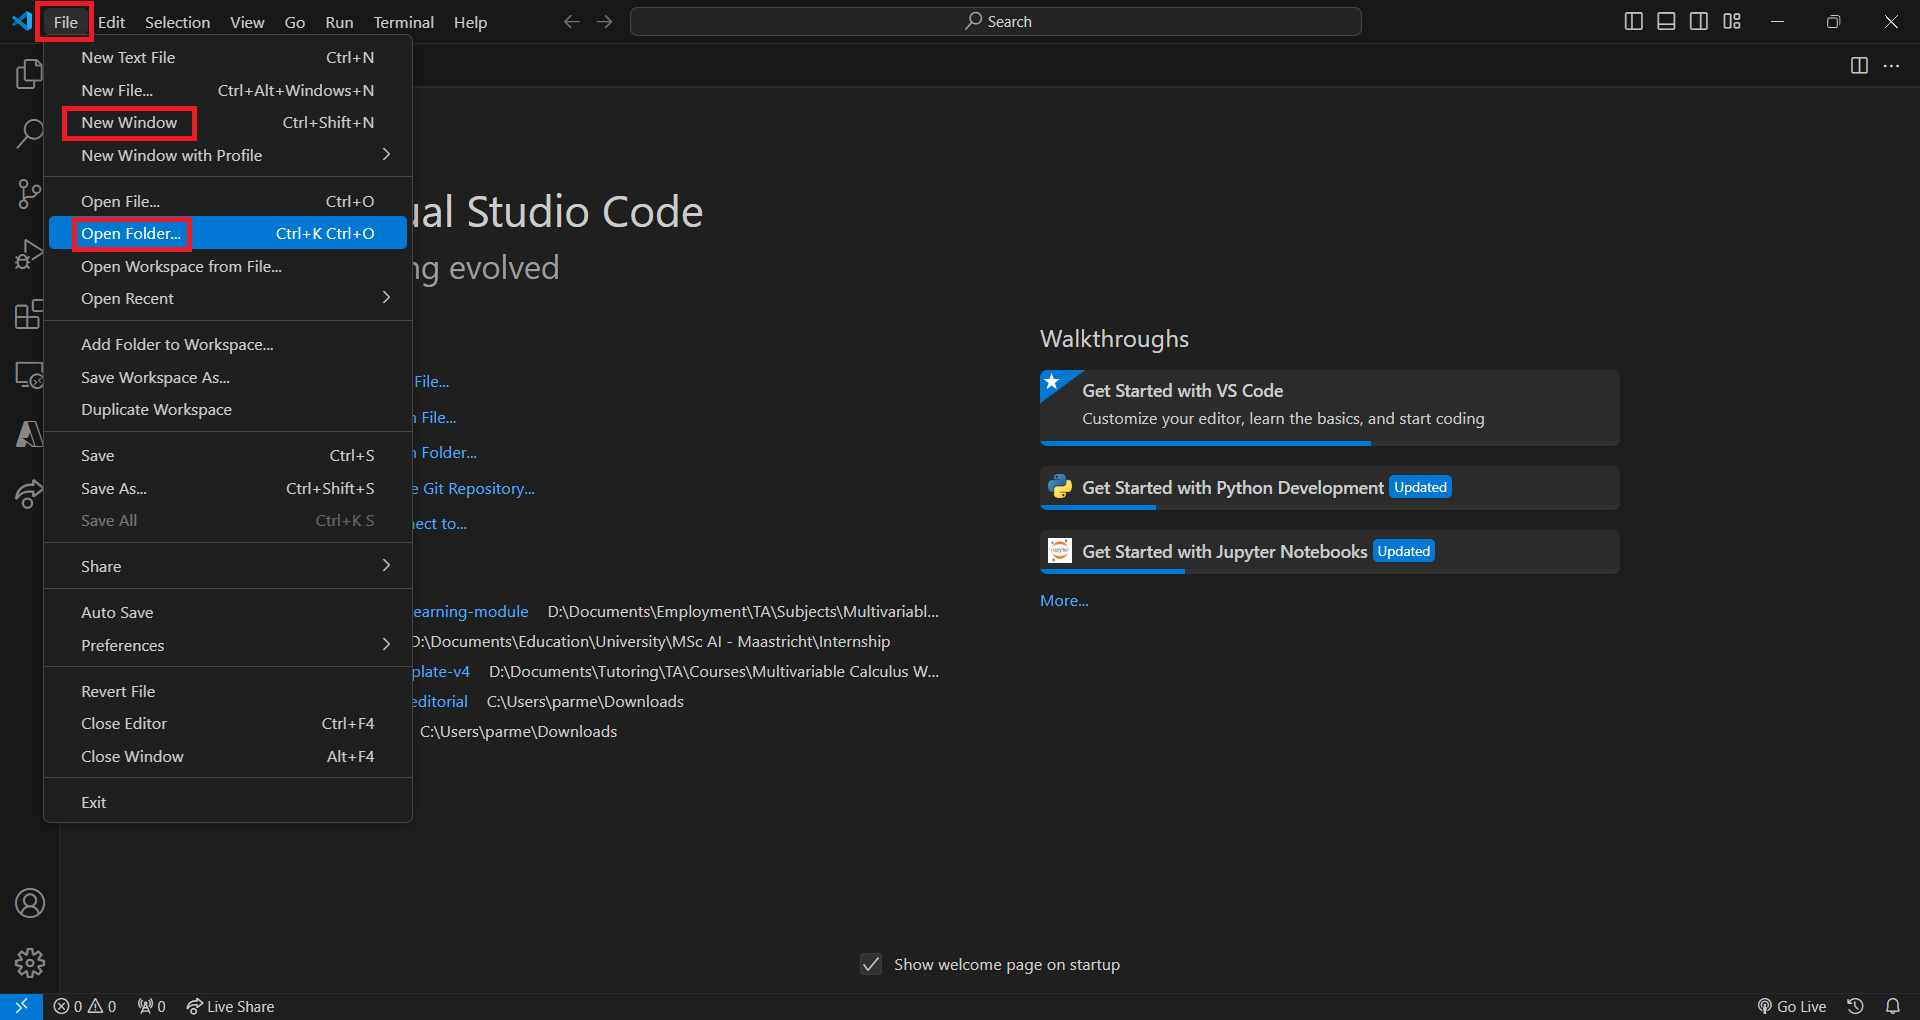
\includegraphics[width=\textwidth]{vscode_open_folder_2.png}
    \caption{Open a new window in VSCode, or open a folder through the \emph{File} menu.}
    \label{fig:vscode_open_folder_2}   
\end{figure}

Finally, if you want a backup option that will always work without opening any new windows, you can click on \emph{File} on the top menu, choose \emph{Open Folder} from the dropdown menu, and search for your folder through the popup File Explorer (e.g.\ \Cref{fig:vscode_open_folder_2}).

\subsubsection{Create a new file within an open folder in VSCode}

I now assume that you have opened a folder in VSCode. In order to see the contents of the folder, click on the file-looking icon on the left sidebar. In order to create a new file in this folder, right click on any empty space on the \emph{Explorer} window that appears on the left, choose \emph{New File\dots}, and write the full name of the file you want to create INCLUDING THE EXTENSION NAME (e.g. \emph{ex\_1001.html} in full, e.g.\ \Cref{fig:vscode_create_file}). 

\begin{figure}[htbp]
    \centering
    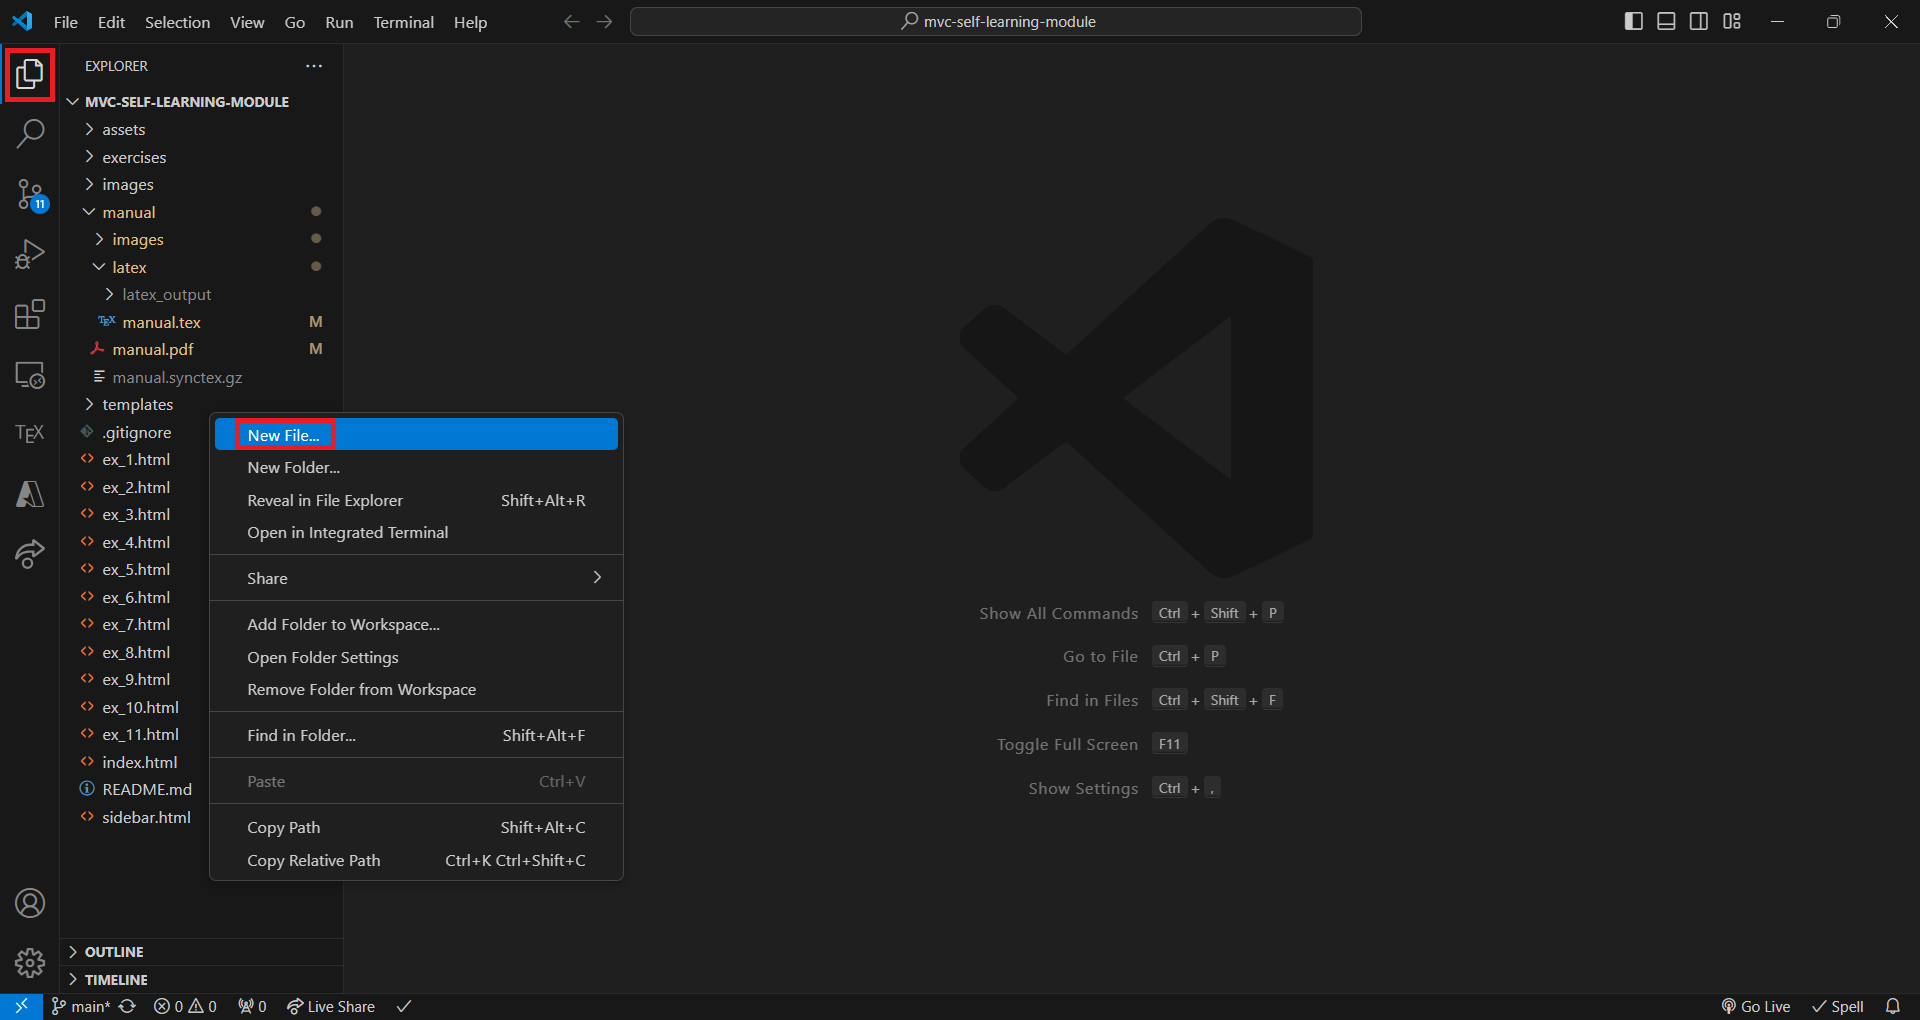
\includegraphics[width=\textwidth]{vscode_create_file.png}
    \caption{Create a file within an open folder VSCode.}
    \label{fig:vscode_create_file}   
\end{figure}

\subsubsection{Edit a file from an open folder in VSCode}

In order to open a file for editing in VSCode, click on the file-looking icon on the left sidebar to open the \emph{Explorer} window, find your file, and DOUBLE CLICK on it to open it for editing. If you click only once, the file will be open for viewing, so if you open a different file immediately afterwards, the previous file will be gone from the main window. The purpose of this is to avoid clutter when you're quickly shuffling through files while looking for something. Having said that, even if you open a file by clicking only once and then you start editing it before opening another file, that also works.

\subsubsection{Format a file in VSCode}

In order to set up formatting options for a file in VSCode, open the file for editing, and then \emph{Right click} $>$ \emph{Format Document With\dots} (e.g.\ \Cref{fig:format_doc}). A popup menu should appear on the top of the main window. If you haven't chosen a formatter before, you can click \emph{Configure Default Formatter\dots} at the bottom of this window, and then choose \emph{Prettier} from the list that will appear (e.g.\ \Cref{fig:configure_formatter}). From that point on, you can format your document anytime by \emph{Right click} $>$ \emph{Format Document} (or by using the shortcut \emph{Shift + Alt + F} if you are willing to remember it).

\begin{figure}[htbp]
    \centering
    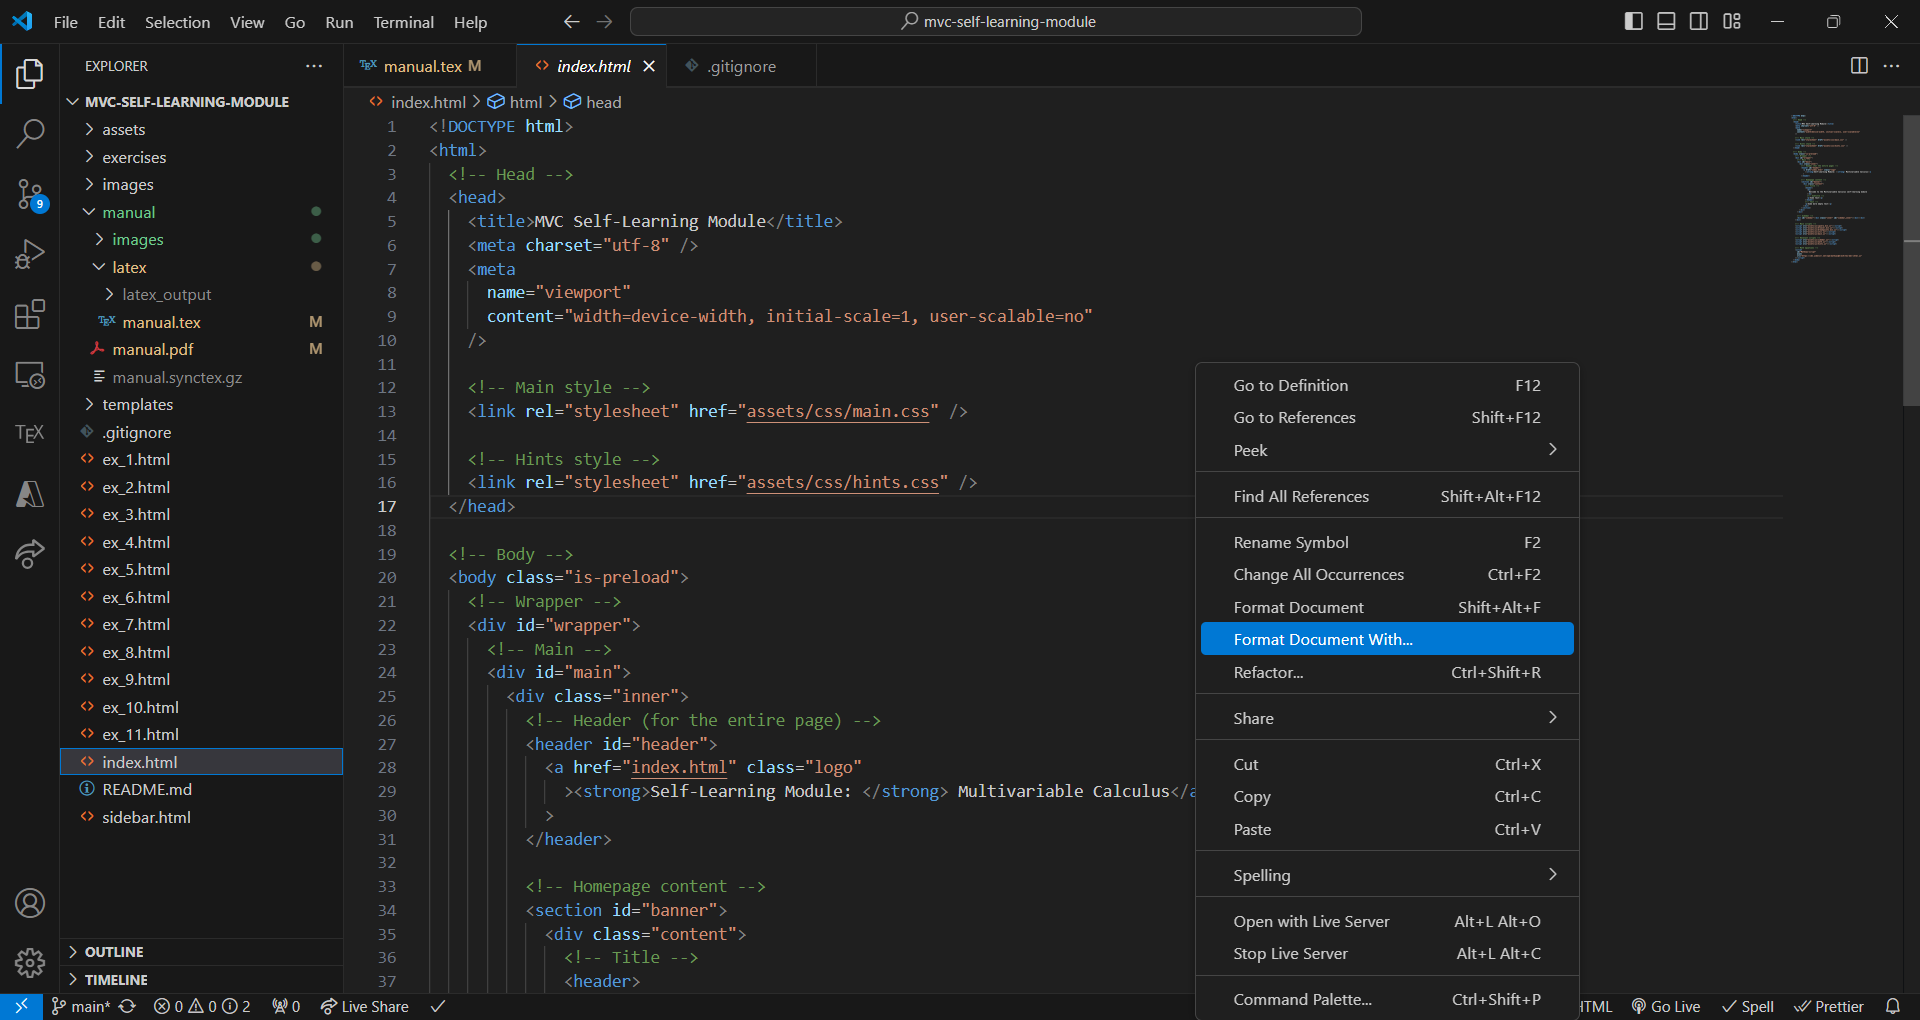
\includegraphics[width=\textwidth]{format_doc.png}
    \caption{\emph{Format Document With\dots}.}
    \label{fig:format_doc}   
\end{figure}

\begin{figure}[htbp]
    \centering
    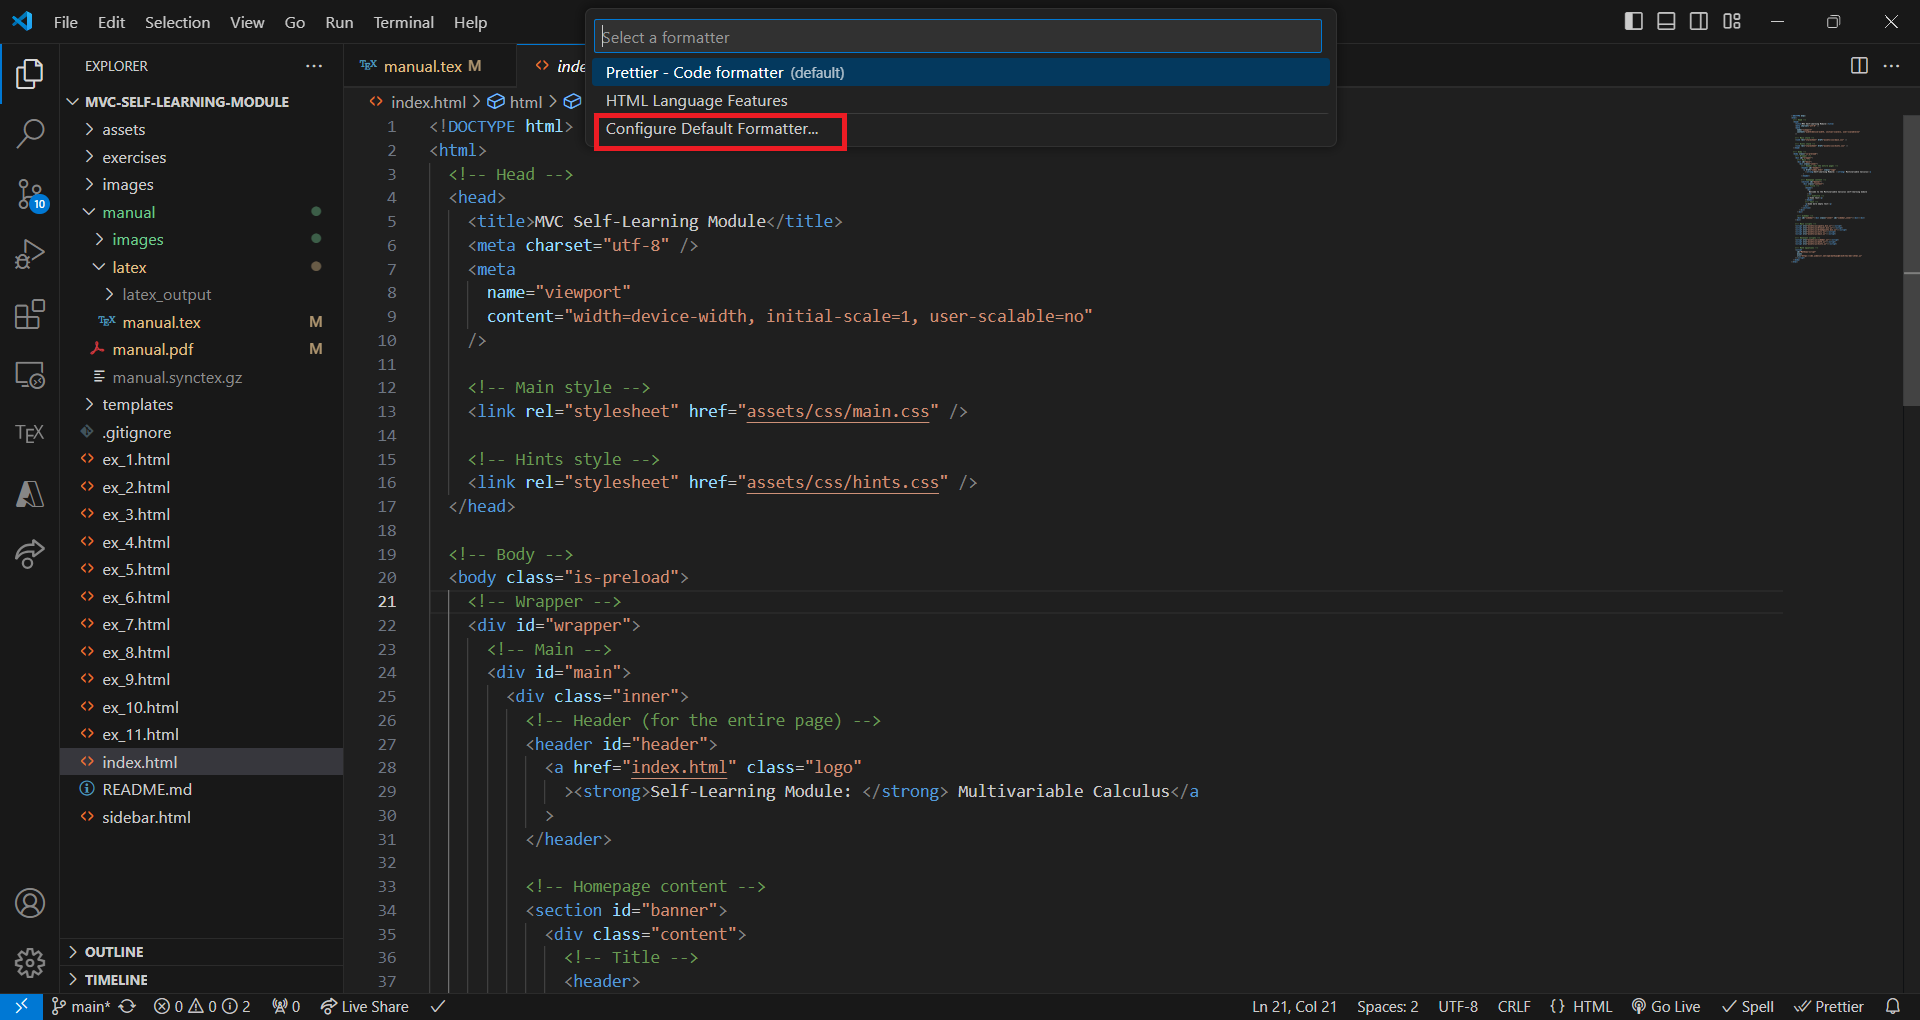
\includegraphics[width=\textwidth]{configure_formatter.png}
    \caption{\emph{Configure Default Formatter\dots}.}
    \label{fig:configure_formatter}   
\end{figure}

\paragraph{Format on save.} I suggest that you set up formatting to happen automatically on save (\emph{Ctrl + S}). It is quicker this way, and even if you accidentally save before you're done and then formatting messes up what you were working on, you can always revert back to the previous state of the document by \emph{Ctrl + Z}, aka \emph{Undo}. To enable format on save, follow the steps:
\begin{enumerate}
    \item Open VSCode settings by \emph{File} (on the top menu) $>$ \emph{Preferences} $>$ \emph{Settings} (e.g.\ \Cref{fig:vscode_settings}).
    \item Click on the \emph{Formatting} bookmark in the main window, scroll down just a bit, and click on \emph{Format On Save} (e.g.\ \Cref{fig:format_on_save}).
\end{enumerate}
You don't need to do anything else to save the settings, the changes should be effective immediately.

\begin{figure}[htbp]
    \centering
    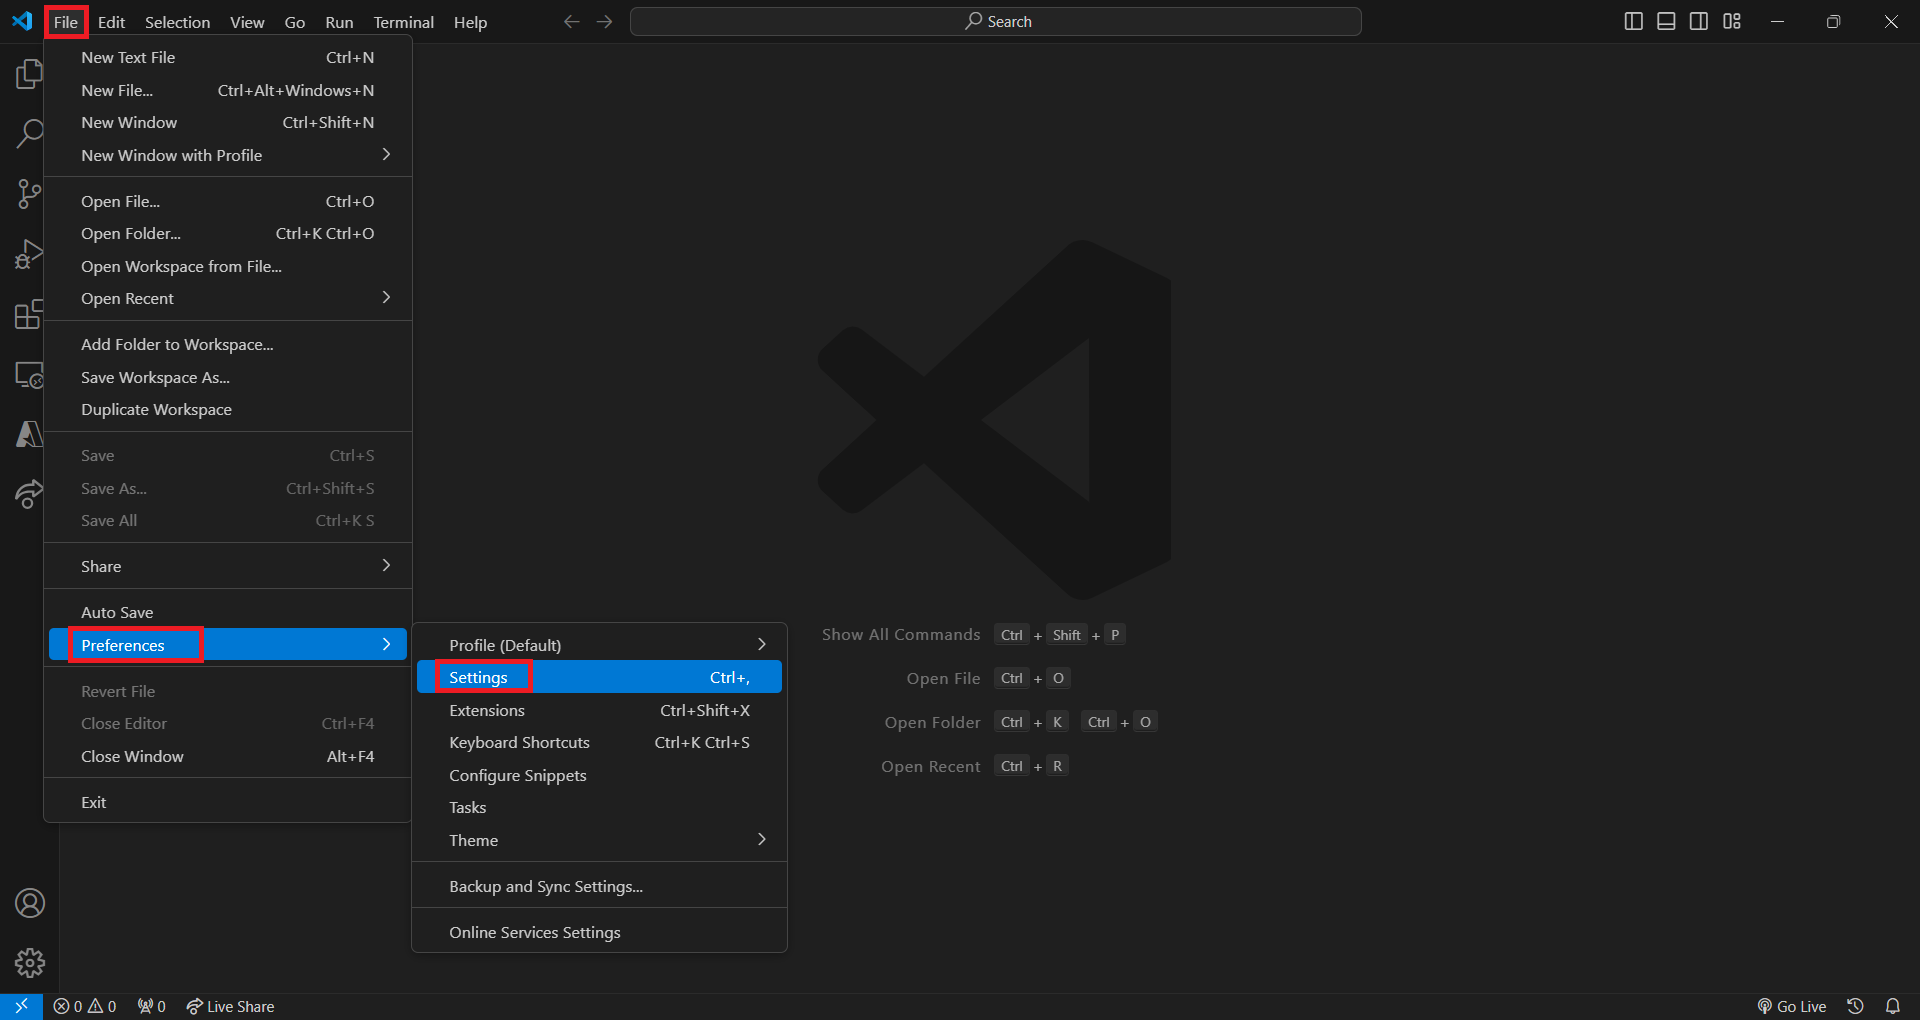
\includegraphics[width=\textwidth]{vscode_settings.png}
    \caption{Open VSCode settings.}
    \label{fig:vscode_settings}   
\end{figure}

\begin{figure}[htbp]
    \centering
    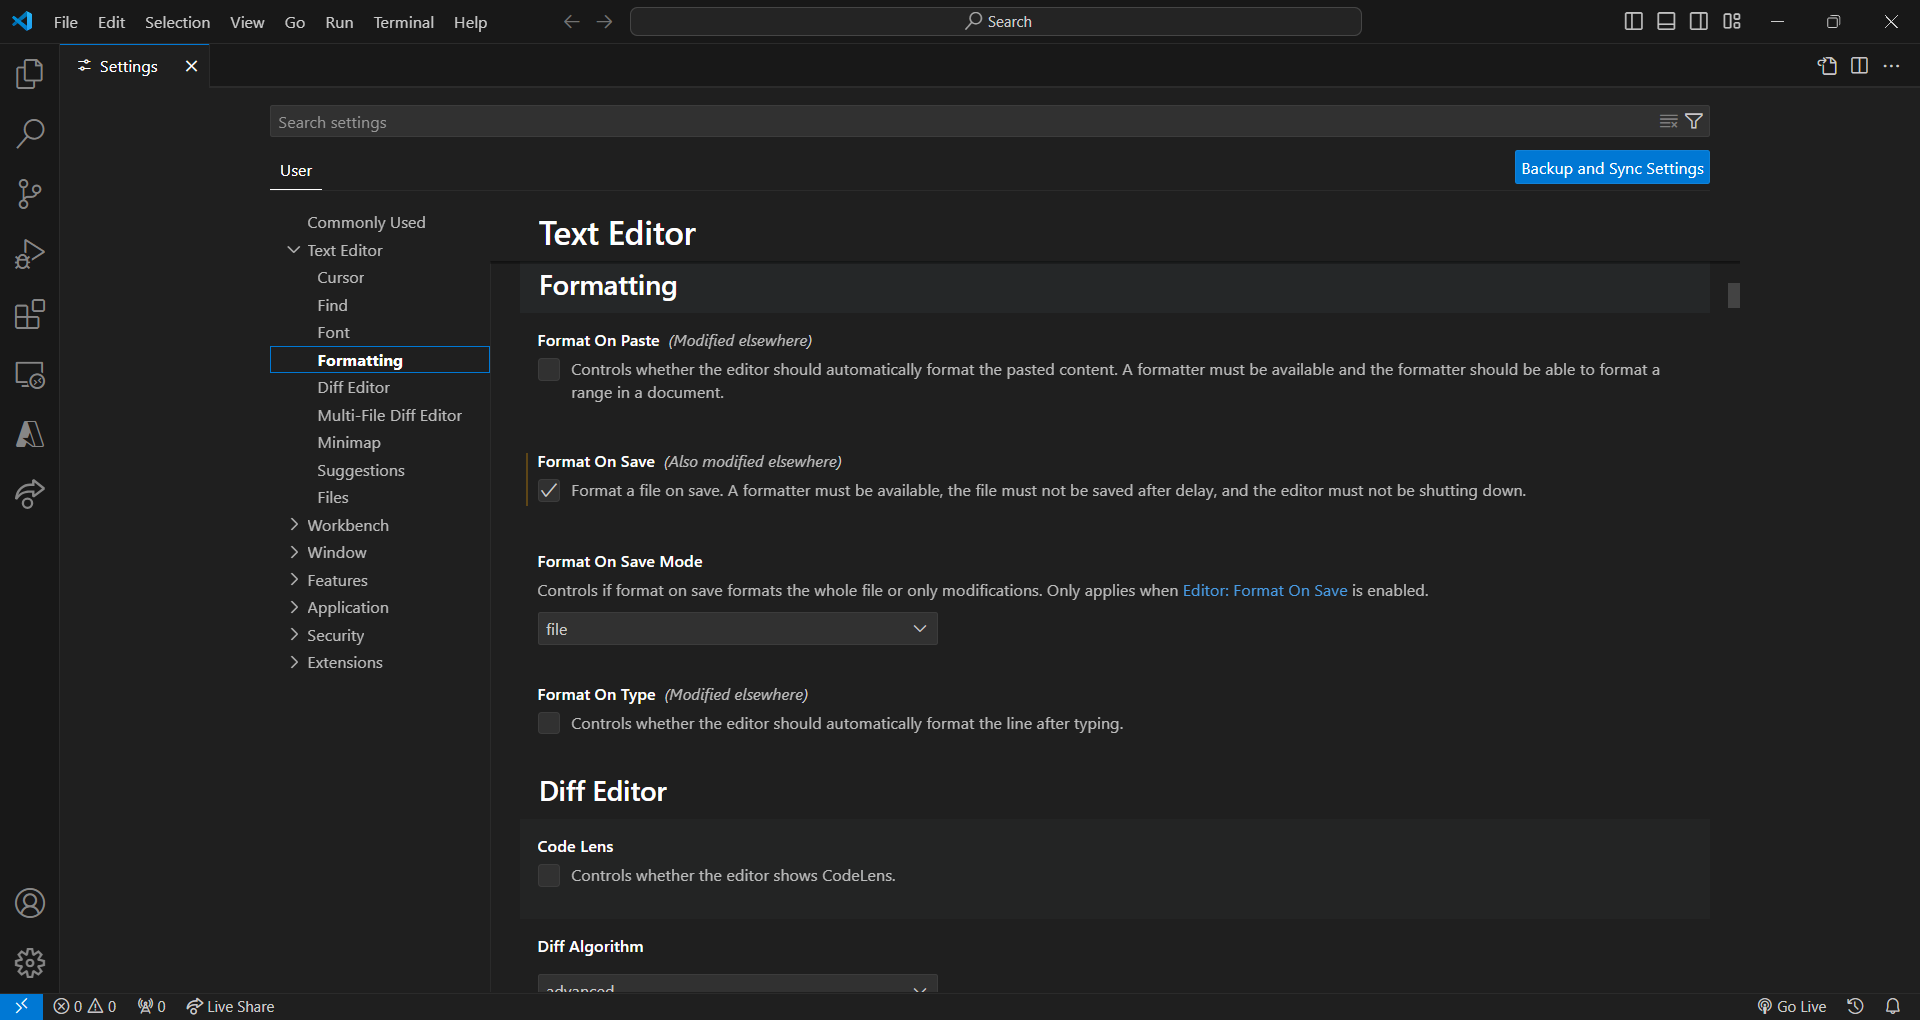
\includegraphics[width=\textwidth]{format_on_save.png}
    \caption{Enable format on save.}
    \label{fig:format_on_save}   
\end{figure}


\subsubsection{Using Live Server}

If you are using VSCode to edit your HTML files, you can run the website on a local live server using the \emph{Live Server} extension (see \Cref{sec:vscode}). All you need to do is click on the \emph{Go Live} option on the bottom menu of VSCode (e.g.\ \Cref{fig:run_live_server}). The local version of the website should open in your default browser in the url (e.g.\ \Cref{fig:website_live_server}):

\url{http://127.0.0.1:5500/}

\begin{figure}[htbp]
    \centering
    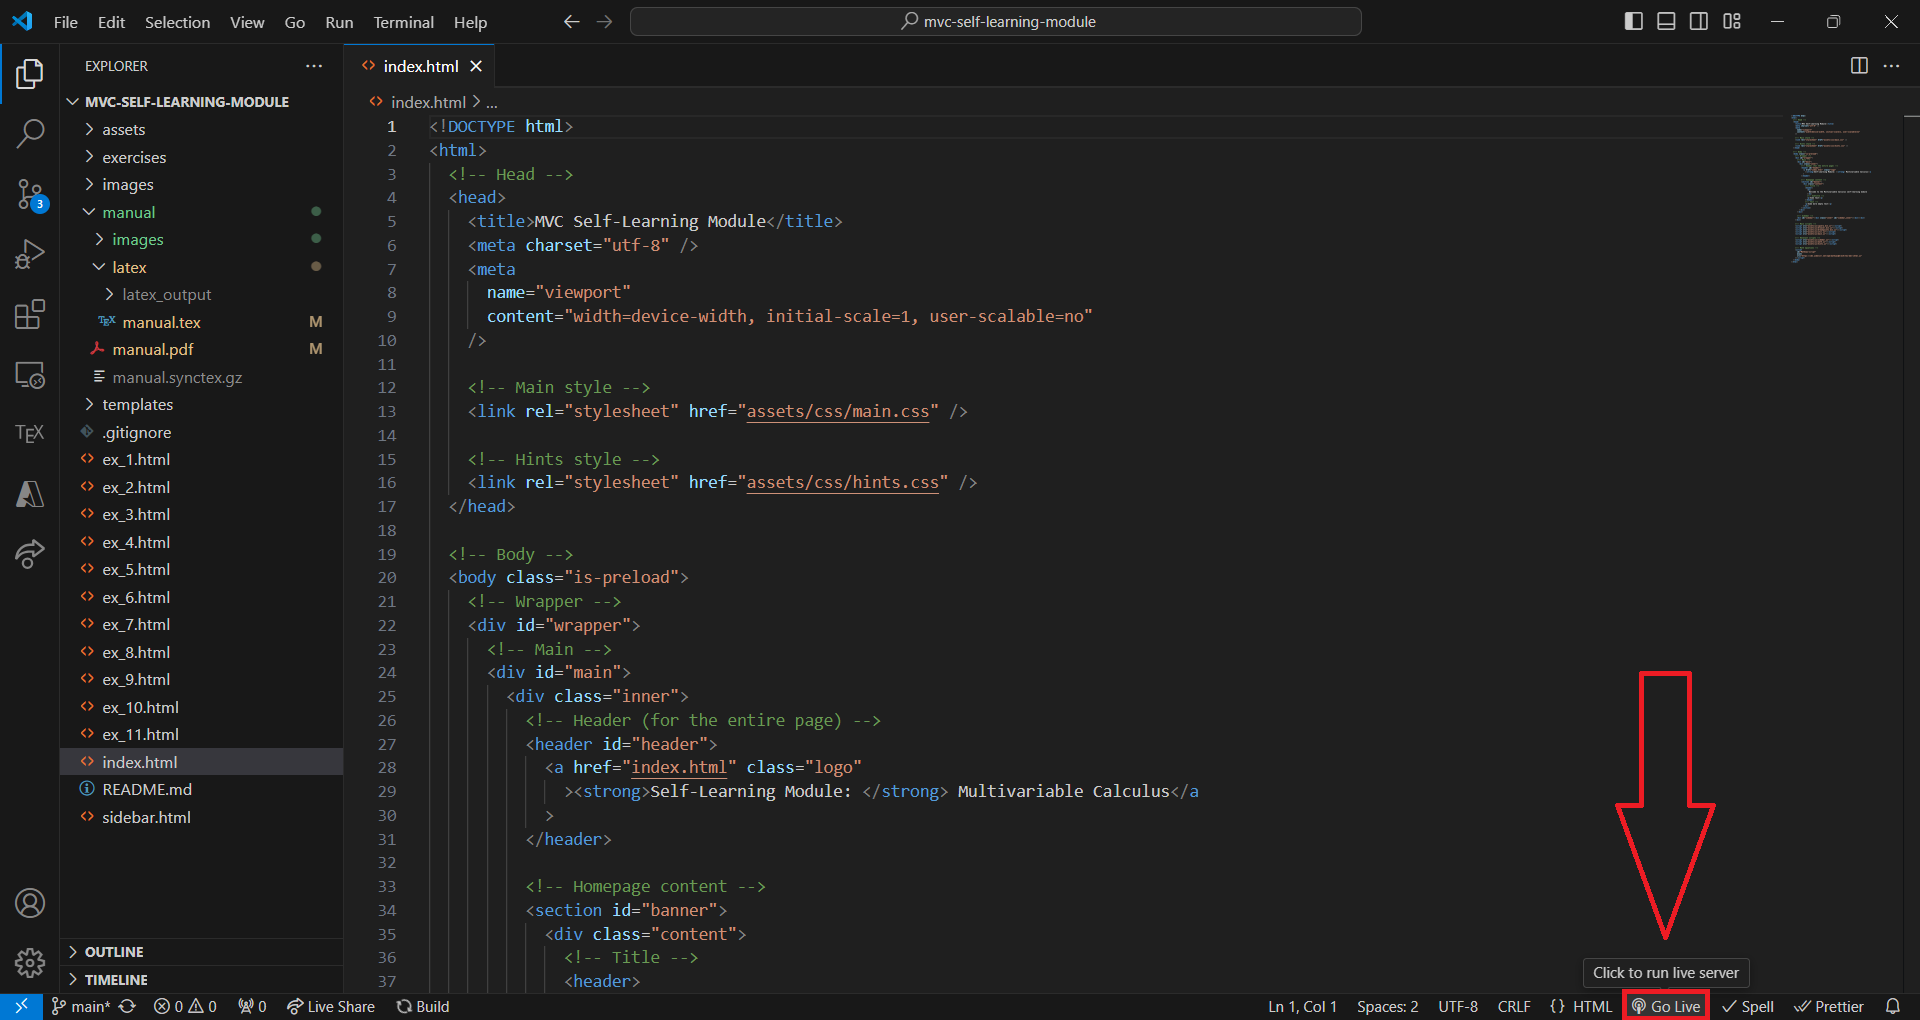
\includegraphics[width=\textwidth]{run_live_server.png}
    \caption{Opening \emph{Live Server} in VSCode.}
    \label{fig:run_live_server}   
\end{figure}

\begin{figure}[htbp]
    \centering
    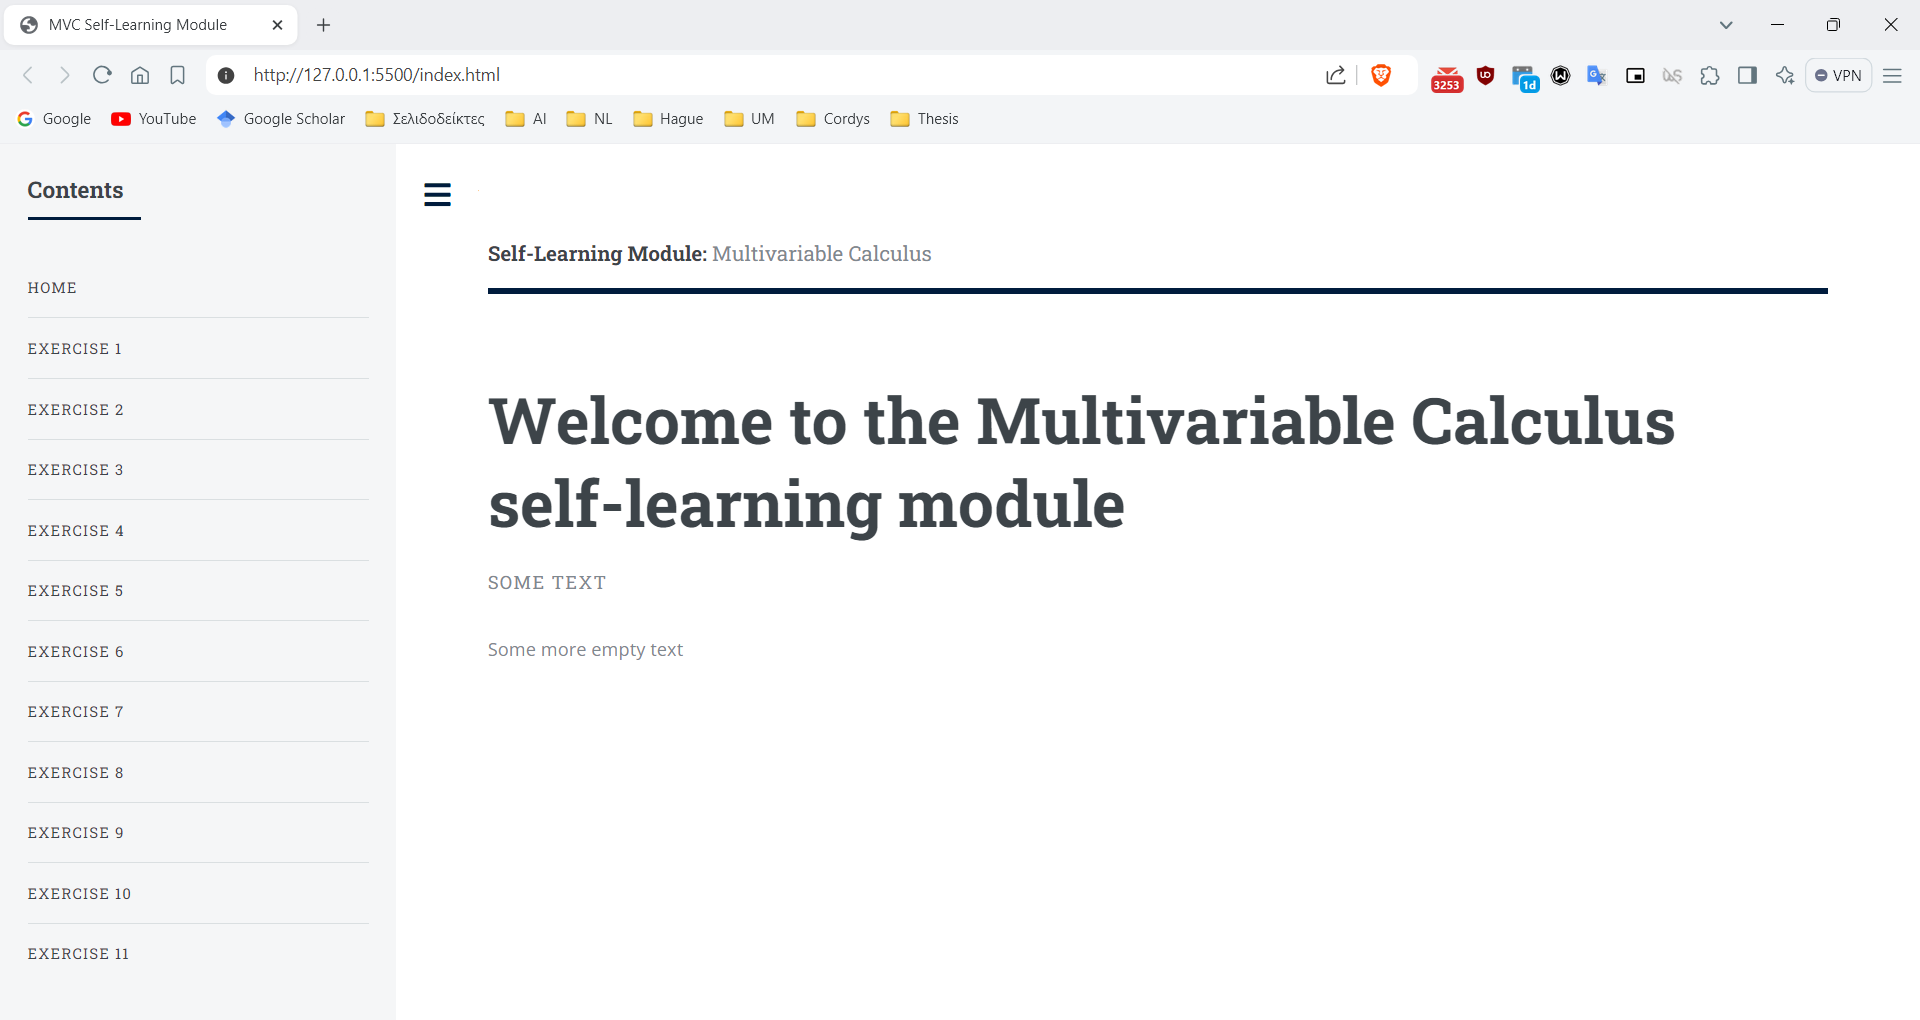
\includegraphics[width=\textwidth]{website_live_server.png}
    \caption{Website running on local live server.}
    \label{fig:website_live_server}   
\end{figure}

\end{document}